% Asal-usul (tidak pernah dicetak): lihat sources/outline_sources.md (Tahun 1: jenis sesar dan teori Anderson; geometri dan klasifikasi lipatan; foliasi, skistositas dan lineasi; mikrostruktur). Nilai soal latihan dan soal dari kalkulator skrap Buku 3 calc/ch17.py; lipatan dan sesar Varden Hills dari figdata/shared/region.py (hanya dibaca). Lipatan, antiklin, sinklin dan sumbu lipatan dimiliki oleh bab 4; lemparan dan pergeseran horizontal oleh bab 5; jurus dan kemiringan garis oleh bab 6; tegangan dan kriteria Coulomb oleh bab 16. Zona geser dan mekanisme deformasi termasuk dalam volume Tahun ke-3 (diceritakan di sini).
\chapter{Sesar, lipatan dan fabrik}\label{ch:b1:faults-folds-fabrics}

Sebuah sayatan jalan memperlihatkan permukaan batuan yang digosok seperti kaca dan tergores alur-alur sejajar yang halus. Di seberang lembah, tebing laut memperlihatkan lapisan batupasir dan batulanau yang melengkung menjadi zigzag dengan sisi-sisi lurus dan sudut-sudut tajam. Di atap dekat sana, batu sabak pecah menjadi lembaran setebal beberapa milimeter, sepanjang bidang yang memotong lapisan lumpur tempat ia dibuat. Masing-masing adalah catatan deformasi batuan, dibaca pada skala yang berbeda: alur-alur memberi arah tempat dua blok saling tergelincir sepanjang sebuah sesar; zigzag mengukur seberapa jauh lapisan dipendekkan; bidang-bidang sabak tumbuh melintasi serat batuan ketika ia diperas. Bab ini memberi geometri yang diperlukan untuk mengukur ketiga catatan itu, dan mekanika bab sebelumnya menjelaskan mengapa sesar mengambil \omterm{def:b1:geological-maps:attitude}{kemiringan} yang mereka miliki.

\begin{recall}
Sikap sebuah bidang adalah \omterm{def:b1:geological-maps:attitude}{arah kemiringan} dan \omterm{def:b1:geological-maps:attitude}{kemiringannya}, ditulis misalnya $080/12$; \omterm{def:b1:geological-maps:attitude}{jurusnya} mengikuti dari kaidah tangan kanan, bidang itu miring ke kanan seorang pengamat yang melihat sepanjang \omterm{def:b1:geological-maps:attitude}{jurus} (\cref{ch:b1:geological-maps}). \omterm{def:b1:geological-maps:fold}{Lipatan} adalah lengkungan lapisan yang tadinya datar; \omterm{def:b1:geological-maps:fold}{antiklin} cembung ke atas dengan batuan tertua di intinya, \omterm{def:b1:geological-maps:fold}{sinklin} cekung ke atas; \omterm{def:b1:geological-maps:fold}{sumbu lipatan} adalah garis tempat lapisan melengkung paling banyak (\cref{ch:b1:geological-maps}). Lemparan dan pergeseran horizontal sebuah sesar adalah komponen vertikal dan horizontal pergeserannya (\cref{ch:b1:cross-sections}). Sebuah garis memiliki \omterm{def:b1:geological-maps:attitude}{jurus} dan \omterm{def:b1:geological-maps:attitude}{kemiringan} garis, dan vektor satuan ke bawah $(\cos p\sin t, \cos p\cos t, -\sin p)$ (\cref{ch:b1:field-lab-methods-1}). Batuan yang mematuhi kriteria Coulomb pecah pada bidang-bidang pada $\ang{45} - \phi/2$ dari $\sigma_1$, dan sesar yang sudah ada tergelincir menurut \omterm{prop:b1:stress-strain-rheology:byerlee}{hukum Byerlee} (\cref{ch:b1:stress-strain-rheology}). Sebuah \omterm{def:b1:rock-forming-minerals:mineral}{mineral} berada dalam pemadaman di antara polarisator bersilang ketika arah getarnya sejajar dengan arah polarisator (\cref{ch:b1:optical-mineralogy}). Sesar telah ditemui di Buku 1, kelas 7; \omterm{def:b1:faults-folds-fabrics:fault-types}{sesar naik}, \omterm{def:b1:faults-folds-fabrics:fault-types}{sesar dorong} dan \omterm{def:b1:faults-folds-fabrics:foliation}{foliasi} di Buku 2, kelas 12. Hasil kali silang dua vektor tegak lurus terhadap keduanya (matematika, Tahun 1).
\end{recall}

\section{Sesar: geometri dan kinematika}\label{sec:b1:faults-folds-fabrics:faults}

Sebuah sesar adalah permukaan tempat dua blok batuan saling tergelincir. Untuk menggambarkan gerakan kita memerlukan nama bagi kedua blok dan bagi pergeseran, serta cara mengukur arahnya di dalam bidang sesar.

\begin{definition}[Dinding gantung dan dinding bawah, vektor geser, pergeseran bersih, rake]\label{def:b1:faults-folds-fabrics:fault-elements}
Anggap sebuah sesar secara lokal adalah bidang yang tidak tegak. \emph{Dinding gantung}\index{dinding gantung} adalah blok di atasnya, \emph{dinding bawah}\index{dinding bawah} blok di bawahnya. Misalkan $A$ adalah titik pada dinding bawah dan $A'$ titik pada dinding gantung yang bersentuhan dengannya sebelum gerakan. \emph{Vektor geser}\index{vektor geser} $\overrightarrow{AA'}$ adalah pergeseran dinding gantung relatif terhadap dinding bawah; panjangnya adalah \emph{pergeseran bersih}\index{pergeseran bersih}. \emph{Rake}\index{rake} $r$ (disebut juga pitch) dari vektor geser adalah sudut, diukur dalam bidang sesar, dari arah \omterm{def:b1:geological-maps:attitude}{jurus} yang diberikan oleh kaidah tangan kanan ke vektor geser, positif ketika vektor geser menunjuk ke atas bidang dan negatif ketika ia menunjuk ke bawahnya: $\ang{-180} < r \le \ang{180}$. Ini adalah konvensi para seismolog, dipakai lagi untuk gempa bumi di \cref{ch:b1:earthquake-source}; banyak ahli geologi lapangan sebaliknya mencatat sudut antara 0 dan \ang{180}, diukur searah jarum jam dari \omterm{def:b1:geological-maps:attitude}{jurus} yang dilihat dari atas, dan menambahkan arah gerakan dengan kata-kata.
\end{definition}
% ledger: ar:rake, ws:rake, ws:fault-terms

Kedua nama itu berasal dari pertambangan: seorang penambang yang bekerja pada urat yang miring berdiri di atas \omterm{def:b1:faults-folds-fabrics:fault-elements}{dinding bawah} dan memiliki \omterm{def:b1:faults-folds-fabrics:fault-elements}{dinding gantung} di atas kepalanya. Pergeseran yang terlihat dalam satu potongan tidak, secara umum, sama dengan pergeseran: lapisan yang tergeser pada peta atau penampang menunjukkan pemisahan, yang bergantung pada sikap lapisan itu. Pergeseran memerlukan dua titik yang dahulunya satu, seperti dua belahan sebuah garis yang dipotong oleh sesar, misalnya tepi sebuah dike terhadap lapisan.

\begin{omfigure}
\begin{tikzpicture}[>={Stealth[length=5pt]}, font=\small]
% (a) the fault plane seen face-on; slip vector of length 3.6 cm at rake -35 deg
% (normal and sinistral): strike-slip component 3.6 cos 35 = 2.949, dip-slip 3.6 sin 35 = 2.065
\pgfmathsetmacro{\Ls}{3.6*cos(35)}\pgfmathsetmacro{\Ld}{3.6*sin(35)}
\begin{scope}
  \fill[omDef!15] (0,0) rectangle (6.2,3.4);
  \draw[omDef, line width=0.7pt] (0,0) rectangle (6.2,3.4);
  \draw[line width=1.2pt] (0,3.4) -- (6.2,3.4);
  \node[anchor=south, font=\scriptsize] at (3.1,3.4) {garis jurus, tempat sesar bertemu tanah};
  \draw[->, line width=0.6pt] (6.45,3.0) -- (6.45,2.0) node[midway, right, font=\scriptsize, align=left] {ke bawah\\ kemiringan};
  \draw[->, line width=0.6pt] (0.3,0.35) -- (1.3,0.35) node[right, font=\scriptsize] {jurus};
  \coordinate (A) at (1.2,2.55);
  \coordinate (B) at ($(A)+(\Ls,0)$);
  \coordinate (A2) at ($(A)+(\Ls,-\Ld)$);
  \draw[omProp, dashed, line width=0.7pt] (A) -- (B) node[midway, above, font=\scriptsize] {komponen pergeseran jurus};
  \draw[omProp, dashed, line width=0.7pt] (B) -- (A2) node[midway, right, font=\scriptsize, align=left] {komponen\\ pergeseran kemiringan};
  \draw[->, line width=1.3pt, omThm] (A) -- (A2) node[midway, below left, font=\scriptsize, inner sep=1pt] {vektor geser};
  \draw[black] ($(A)+(0.9,0)$) arc[start angle=0, end angle=-35, radius=0.9];
  \node[font=\scriptsize] at ($(A)+(-17.5:1.15)$) {$r$};
  \fill (A) circle[radius=1.4pt] node[above left, inner sep=1.5pt] {$A$};
  \fill (A2) circle[radius=1.4pt] node[below right, inner sep=1.5pt] {$A'$};
  \node[font=\small\bfseries] at (3.1,-0.55) {(a) dalam bidang sesar};
\end{scope}
% (b) the vertical section through the dip line: dip 50 deg; dip-slip 2.065 -> throw 1.582, heave 1.327
\begin{scope}[xshift=9.4cm, yshift=0.2cm]
  \pgfmathsetmacro{\th}{\Ld*sin(50)}\pgfmathsetmacro{\he}{\Ld*cos(50)}
  \fill[omLithSand!40] (-1.2,0) -- (-1.2,3.2) -- (0,3.2) -- ({3.2/tan(50)},0) -- cycle;
  \fill[omLithSand!20] ({3.2/tan(50)},0) -- (0,3.2) -- (4.2,3.2) -- (4.2,0) -- cycle;
  \draw[line width=0.6pt] (-1.2,3.2) -- (4.2,3.2);
  \draw[omDef, line width=1.1pt] (0,3.2) -- ({3.2/tan(50)},0);
  \draw[black] (0.75,3.2) arc[start angle=0, end angle=-50, radius=0.75];
  \node[font=\scriptsize] at ($(0,3.2)+(-25:1.0)$) {$\delta$};
  \coordinate (P) at ({1.3*cos(50)},{3.2-1.3*sin(50)});
  \coordinate (Q) at ($(P)+({\Ld*cos(50)},{-\Ld*sin(50)})$);
  \coordinate (R) at ($(P)+(\he,0)$);
  \draw[->, omProp, line width=1.1pt] (P) -- (Q);
  \draw[black!80, densely dotted, line width=0.7pt] (P) -- (R) node[midway, above, font=\scriptsize] {pergeseran horizontal};
  \draw[black!80, densely dotted, line width=0.7pt] (R) -- (Q) node[midway, right, font=\scriptsize] {lemparan};
  \node[font=\scriptsize, omProp, anchor=east] at ($(P)!0.55!(Q)+(-0.08,0)$) {pergeseran kemiringan};
  \node[font=\small] at (3.3,2.6) {dinding gantung};
  \node[font=\small] at (-0.55,1.0) {dinding bawah};
  \node[font=\small\bfseries] at (1.5,-0.75) {(b) dalam bidang vertikal kemiringan};
\end{scope}
\end{tikzpicture}
\par\smallskip{\small Unsur-unsur sebuah sesar, digambar sesuai skala untuk sesar yang miring $\delta = \ang{50}$ dan \omterm{def:b1:faults-folds-fabrics:fault-elements}{vektor geser} dengan \omterm{def:b1:faults-folds-fabrics:fault-elements}{rake} $r = \ang{-35}$. (a) Bidang sesar dilihat dari depan: \omterm{def:b1:faults-folds-fabrics:fault-elements}{vektor geser} $\overrightarrow{AA'}$ terbagi menjadi komponen sepanjang \omterm{def:b1:geological-maps:attitude}{jurus} dan satu ke bawah \omterm{def:b1:geological-maps:attitude}{kemiringan}. (b) Penampang vertikal tegak lurus terhadap \omterm{def:b1:geological-maps:attitude}{jurus}: komponen pergeseran \omterm{def:b1:geological-maps:attitude}{kemiringan} terbagi menjadi lemparan dan pergeseran horizontal.}
\label{fig:b1:faults-folds-fabrics:elements}
\end{omfigure}

\begin{proposition}[Komponen pergeseran]\label{prop:b1:faults-folds-fabrics:slip-components}
Anggap sebuah sesar memiliki \omterm{def:b1:geological-maps:attitude}{arah kemiringan} $\alpha$ dan \omterm{def:b1:geological-maps:attitude}{kemiringan} $\delta$, dan \omterm{def:b1:faults-folds-fabrics:fault-elements}{vektor geser} dengan panjang $L$ dan \omterm{def:b1:faults-folds-fabrics:fault-elements}{rake} $r$. Dengan komponen timur, utara dan atas, misalkan $\mathbf s = (\sin(\alpha-\ang{90}), \cos(\alpha-\ang{90}), 0)$ menjadi vektor satuan sepanjang \omterm{def:b1:geological-maps:attitude}{jurus} dan $\mathbf u = (-\cos\delta\sin\alpha,
-\cos\delta\cos\alpha, \sin\delta)$ vektor satuan ke atas \omterm{def:b1:geological-maps:attitude}{kemiringan}. Maka
\[
  \overrightarrow{AA'} = L\,(\cos r\,\mathbf s + \sin r\,\mathbf u),
\]
komponen pergeseran \omterm{def:b1:geological-maps:attitude}{jurusnya} adalah $L\cos r$ dan komponen pergeseran \omterm{def:b1:geological-maps:attitude}{kemiringannya} $L\sin r$; lemparannya $L\,|\sin r|\sin\delta$, pergeseran horizontalnya $L\,|\sin r|\cos\delta$, dan \omterm{def:b1:faults-folds-fabrics:fault-elements}{vektor geser} menunjam sebesar $p$ dengan $\sin p = |\sin r|\sin\delta$.
\end{proposition}

\begin{proof}
Vektor $\mathbf s$ horizontal dan menunjuk sepanjang \omterm{def:b1:geological-maps:attitude}{jurus}; $\mathbf u$ adalah kebalikan dari vektor satuan ke bawah pada garis \omterm{def:b1:geological-maps:attitude}{kemiringan}, yang memiliki arah $\alpha$ dan \omterm{def:b1:field-lab-methods-1:trend-plunge}{penunjaman} $\delta$ (\cref{ch:b1:field-lab-methods-1}). Keduanya terletak dalam bidang sesar, dan $\mathbf s\cdot\mathbf u = -\cos\delta(\sin(\alpha -
\ang{90})\sin\alpha + \cos(\alpha - \ang{90})\cos\alpha) = -\cos\delta\cos\ang{90} = 0$,
sehingga keduanya membentuk basis ortonormal bidang itu. Sebuah vektor bidang dengan panjang $L$ pada sudut $r$ dari $\mathbf s$, dihitung menuju $\mathbf u$, adalah $L(\cos r\,\mathbf s + \sin r\,\mathbf u)$. Komponen vertikalnya adalah $L\sin r\sin\delta$, yang besarnya adalah lemparan; bagian horizontalnya melintasi \omterm{def:b1:geological-maps:attitude}{jurus} adalah $L\sin r$ kali bagian horizontal $\mathbf u$, yang panjangnya $\cos\delta$, yaitu pergeseran horizontal; dan sinus \omterm{def:b1:field-lab-methods-1:trend-plunge}{penunjamannya} adalah komponen vertikalnya dibagi $L$.
\end{proof}

Untuk sesar \omterm{def:b1:geological-maps:attitude}{pergeseran-kemiringan}, $|\sin r| = 1$ dan pergeseran horizontalnya adalah lemparan dibagi $\tan\delta$, seperti di \cref{ch:b1:cross-sections}. \omterm{def:b1:faults-folds-fabrics:fault-elements}{Rake} memilah sesar menjadi keluarga-keluarga.

\begin{definition}[Sesar normal, sesar naik, sesar dorong, sesar geser-mendatar dan sesar geser-miring]\label{def:b1:faults-folds-fabrics:fault-types}
Sebuah sesar yang \omterm{def:b1:faults-folds-fabrics:fault-elements}{vektor gesernya} terletak sepanjang garis \omterm{def:b1:geological-maps:attitude}{kemiringan} ($r = \pm\ang{90}$) adalah sesar \omterm{def:b1:geological-maps:attitude}{pergeseran-kemiringan}: sebuah \emph{sesar normal}\index{sesar normal} ketika \omterm{def:b1:faults-folds-fabrics:fault-elements}{dinding gantung} telah bergerak turun ($r = \ang{-90}$), sebuah \emph{sesar naik}\index{sesar naik} ketika ia telah bergerak naik ($r = \ang{90}$). Sebuah \emph{sesar dorong}\index{sesar dorong} adalah sesar naik yang miring \ang{45} atau kurang. Sebuah sesar yang pergeserannya sejajar dengan \omterm{def:b1:geological-maps:attitude}{jurusnya} ($r = 0$ atau \ang{180}) adalah \emph{sesar geser-mendatar}\index{sesar geser-mendatar}; sesar seperti itu biasanya hampir tegak. Sebuah sesar geser-mendatar adalah \emph{dekstral}\index{dekstral} (geser-kanan) ketika pengamat yang berdiri di salah satu sisinya melihat sisi lain bergeser ke kanan, \emph{sinistral}\index{sinistral} (geser-kiri) ketika ke kiri. Sebuah sesar yang pergeserannya memiliki komponen geser-mendatar dan komponen \omterm{def:b1:geological-maps:attitude}{pergeseran-kemiringan} adalah \emph{sesar geser-miring}\index{sesar geser-miring}; dalam praktik sebuah sesar dinamai menurut komponennya yang lebih besar, sehingga \omterm{def:b1:faults-folds-fabrics:fault-elements}{rake} di dekat \ang{-90} disebut normal.
\end{definition}
% ledger: usgs:fault-types, ws:fault-terms, ar:rake

\begin{proposition}[Arah sesar geser-mendatar]\label{prop:b1:faults-folds-fabrics:sense}
Arah sebuah \omterm{def:b1:faults-folds-fabrics:fault-types}{sesar geser-mendatar} tidak bergantung pada sisi tempat pengamat berdiri. \omterm{def:b1:faults-folds-fabrics:fault-elements}{Rake} dekat $0$ adalah \omterm{def:b1:faults-folds-fabrics:fault-types}{sinistral}, \omterm{def:b1:faults-folds-fabrics:fault-elements}{rake} dekat \ang{180} \omterm{def:b1:faults-folds-fabrics:fault-types}{dekstral}.
\end{proposition}

\begin{proof}
Jika pengamat pada blok 1 melihat blok 2 bergerak sebesar $\mathbf v$, pengamat pada blok 2 melihat blok 1 bergerak sebesar $-\mathbf v$. Berbalik untuk menghadap blok 1, pengamat kedua telah menukar kiri dan kanan. Kedua perubahan itu saling meniadakan: keduanya melihat sisi lain bergerak ke arah yang sama, ke kanan atau ke kiri. Untuk bagian kedua, berdirilah di \omterm{def:b1:faults-folds-fabrics:fault-elements}{dinding bawah} dan hadapkan \omterm{def:b1:faults-folds-fabrics:fault-elements}{dinding gantung}: seseorang kemudian melihat ke \omterm{def:b1:geological-maps:attitude}{arah kemiringan}, dan karena bidang itu miring ke kanan \omterm{def:b1:geological-maps:attitude}{jurusnya}, arah \omterm{def:b1:geological-maps:attitude}{jurus} menunjuk ke kiri seseorang. \omterm{def:b1:faults-folds-fabrics:fault-elements}{Rake} $0$ menggerakkan \omterm{def:b1:faults-folds-fabrics:fault-elements}{dinding gantung} sepanjang \omterm{def:b1:geological-maps:attitude}{jurus}, ke kiri; \omterm{def:b1:faults-folds-fabrics:fault-elements}{rake} \ang{180} menggerakkannya ke kanan.
\end{proof}

Permukaan sesar sering kali sendiri merupakan catatan gerakan: goresan dan serat di atasnya terletak sepanjang pergeseran. Di sekitar permukaan itu, zona sesar mungkin terisi batuan yang pecah oleh gerakan.

\begin{definition}[Cermin sesar, gores garis, batuan sesar]\label{def:b1:faults-folds-fabrics:fault-rocks}
\emph{Gores garis}\index{gores garis} adalah goresan atau serat pada permukaan sesar, sejajar dengan pergeseran; \emph{cermin sesar}\index{cermin sesar} adalah permukaan sesar yang membawanya, sering kali dihaluskan oleh pergeseran. \emph{Batuan sesar}\index{batuan sesar} adalah batuan yang dibuat oleh gerakan pada sesar. \emph{Breksi sesar}\index{breksi sesar} terbuat dari pecahan bersudut dari dinding sesar, diputar dan dipindahkan dari tempatnya, dari blok-blok yang sangat besar hingga sekitar \qty{2}{mm}; \emph{kataklasit}\index{kataklasit} terbuat dari pecahan seukuran pasir atau lebih kecil; keduanya tidak memiliki fabrik, pecahannya terletak secara acak. \emph{Gouge sesar}\index{gouge sesar} adalah batuan sesar yang kaya lempung, sangat lunak di \omterm{def:b1:geological-maps:geological-map}{singkapan}. \emph{Milonit}\index{milonit} adalah batuan berbutir halus dan berfoliasi kuat yang dibuat di zona geser oleh penggeseran duktil, butirannya mengecil oleh rekristalisasi alih-alih oleh penggilingan.
\end{definition}
% ledger: ws:fault-terms, ws:fault-rocks

\omterm{def:b1:faults-folds-fabrics:fault-rocks}{Batuan sesar} adalah pengukur kedalaman, dan mereka mengikuti \omterm{def:b1:stress-strain-rheology:strength-envelope}{amplop kekuatan} \cref{ch:b1:stress-strain-rheology}. Gouge, breksi dan \omterm{def:b1:faults-folds-fabrics:fault-rocks}{kataklasit}, dengan fabriknya yang acak, dibuat oleh tergelincir gesek dan rekahan di \omterm{def:b1:layered-earth:layers}{kerak} rapuh; \omterm{def:b1:faults-folds-fabrics:fault-rocks}{milonit} dibuat di bawah \omterm{def:b1:stress-strain-rheology:strength-envelope}{transisi rapuh--duktil}, tempat sesar berlanjut ke bawah sebagai pita geser duktil. Untuk \omterm{def:b1:heat-budget:geotherm}{geoterm} normal dan air yang cukup, transisi di antara keduanya terletak pada \qtyrange{10}{15}{km}, dekat dengan \qty{13.7}{km} amplop bab sebelumnya, dan sesar paling kuat di sana. Di sepanjang sesar besar yang dibawa naik dari kedalaman, urutan yang sama ditemukan berdampingan: zona gouge dekat permukaan, lalu \omterm{def:b1:faults-folds-fabrics:fault-rocks}{kataklasit}, lalu \omterm{def:b1:faults-folds-fabrics:fault-rocks}{milonit}. Nama \omterm{def:b1:faults-folds-fabrics:fault-rocks}{milonit}, dari kata Yunani untuk menggiling tepung, mencatat suatu kekeliruan: dahulu dikira batuan yang digiling. Volume Tahun ke-3 mempelajari zona geser dalam itu dan mekanisme yang membuat \omterm{def:b1:faults-folds-fabrics:fault-rocks}{milonit}.
% ledger: sibson:fault-rocks, sibson:alpine-fault, ws:fault-rocks

\begin{omfigure}
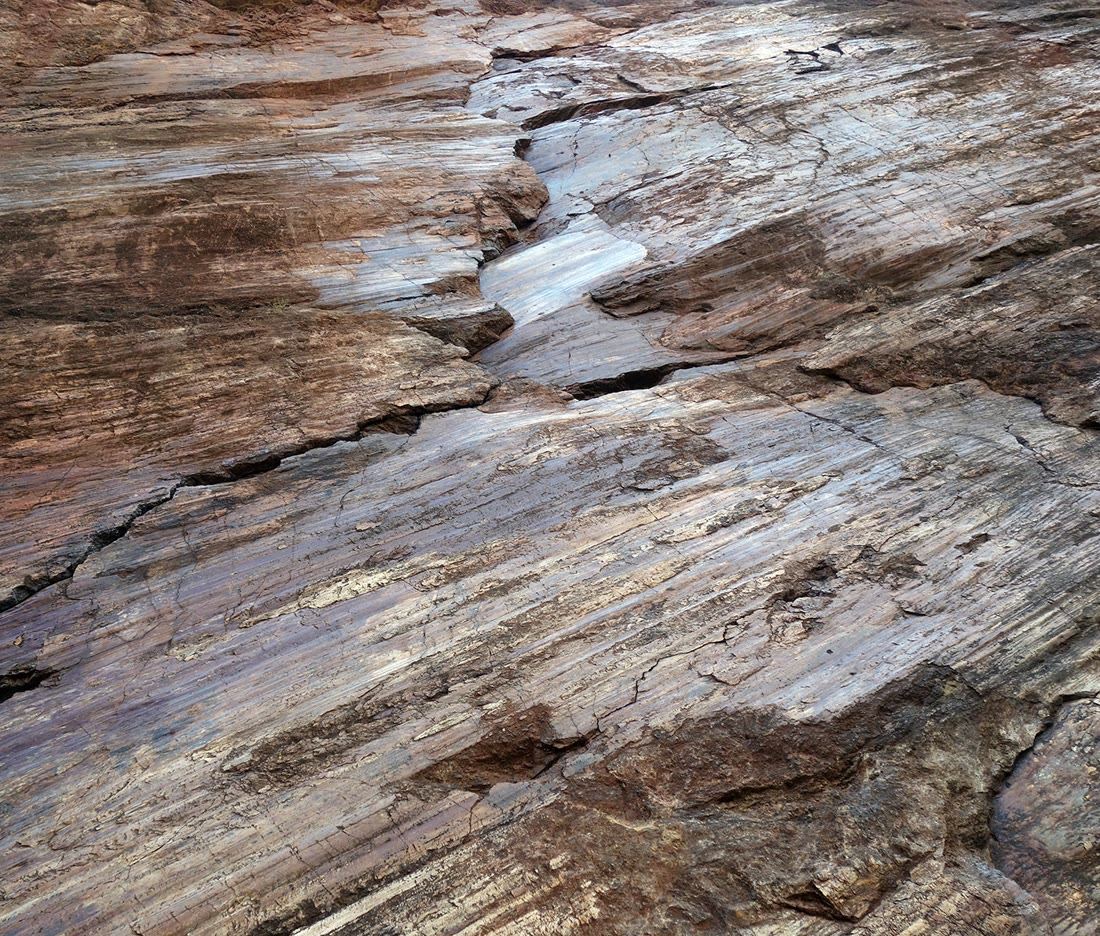
\includegraphics[height=5.2cm]{images/book3/b1-slickenside.jpg}\hfill
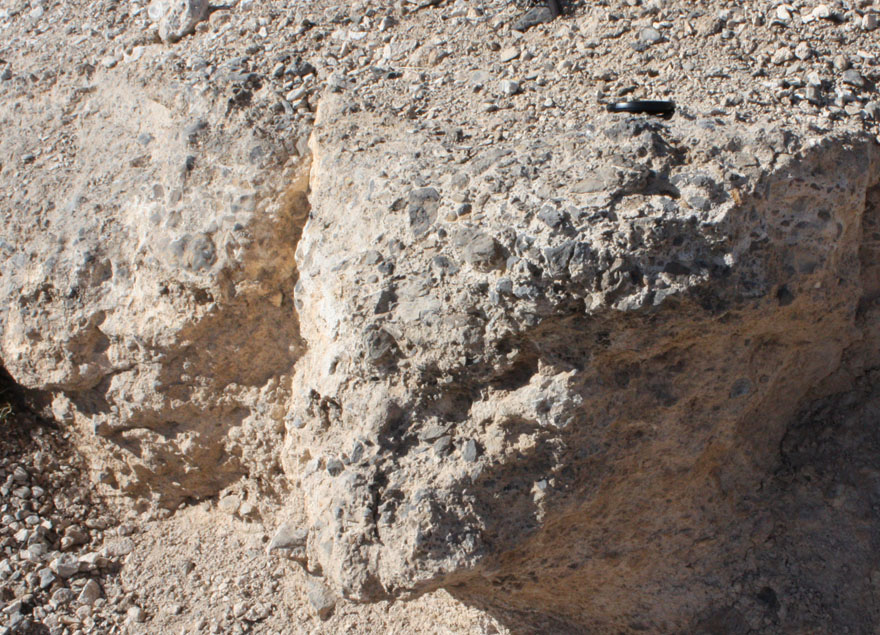
\includegraphics[height=5.2cm]{images/book3/b1-fault-breccia.jpg}
\par\smallskip{\small Kiri: sebuah \omterm{def:b1:faults-folds-fabrics:fault-rocks}{cermin sesar} pada permukaan sesar dalam rijang, sekitar \qtyproduct{3 x 3}{m} dari permukaan setinggi \qty{10}{m}, Corona Heights, San Francisco; permukaan yang digosok itu bergaris-garis sepanjang pergeseran. Foto: Dextersinister, CC~BY-SA~4.0. Kanan: \omterm{def:b1:faults-folds-fabrics:fault-rocks}{breksi sesar} dari Keystone Thrust, Red Rock Canyon, Nevada: pecahan bersudut batuan karbonat kelabu dalam matriks yang lebih pucat; tutup lensa di kanan atas berdiameter \qty{5.8}{cm}. Foto: Jstuby, domain publik. Keduanya dari Wikimedia Commons.}
\label{fig:b1:faults-folds-fabrics:fault-surfaces}
\end{omfigure}
% ledger: commons:slickenside, commons:breccia

\begin{method}[Mengukur pergeseran pada sesar]\label{met:b1:faults-folds-fabrics:slip}
\begin{enumerate}
  \item Ukur sikap $\alpha/\delta$ permukaan sesar dan tulis \omterm{def:b1:geological-maps:attitude}{jurusnya}, $\alpha - \ang{90}$.
  \item Ukur \omterm{def:b1:faults-folds-fabrics:fault-rocks}{gores garis}: \omterm{def:b1:faults-folds-fabrics:fault-elements}{rake-nya} pada sesar, atau \omterm{def:b1:geological-maps:attitude}{jurus} dan \omterm{def:b1:field-lab-methods-1:trend-plunge}{penunjamannya}; untuk \omterm{def:b1:faults-folds-fabrics:fault-elements}{rake} $r$, $\sin p = |\sin r|\sin\delta$.
  \item Cari arah gerak \omterm{def:b1:faults-folds-fabrics:fault-elements}{dinding gantung}, dari penanda yang tergeser melintasi sesar, dan beri \omterm{def:b1:faults-folds-fabrics:fault-elements}{rake} tandanya: negatif jika \omterm{def:b1:faults-folds-fabrics:fault-elements}{dinding gantung} turun.
  \item Cari \omterm{def:b1:faults-folds-fabrics:fault-elements}{pergeseran bersih} $L$ dari dua titik yang dahulunya satu; jika hanya lemparan $h$ dari penanda horizontal yang diketahui, $L = h/(|\sin r|\sin\delta)$.
  \item Hitung komponen-komponennya dengan \cref{prop:b1:faults-folds-fabrics:slip-components} dan beri nama sesarnya dengan \cref{def:b1:faults-folds-fabrics:fault-types}.
\end{enumerate}
\end{method}

\begin{inthefield}[Mengukur permukaan sesar]
Seorang geolog yang menemukan permukaan sesar di \omterm{def:b1:geological-maps:geological-map}{singkapan} mengukurnya seperti bidang lain, dengan kompas-klinometer yang diletakkan di atas permukaan, lalu mengukur \omterm{def:b1:faults-folds-fabrics:fault-rocks}{gores garis} di atasnya, baik sebagai \omterm{def:b1:faults-folds-fabrics:fault-elements}{rake}, dengan busur derajat yang diletakkan pada bidang, maupun sebagai \omterm{def:b1:geological-maps:attitude}{jurus} dan \omterm{def:b1:field-lab-methods-1:trend-plunge}{penunjaman}. Keduanya diperiksa satu sama lain dengan rumus langkah 2 metode itu. Arah gerakan adalah bagian yang sulit. Langkah-langkah kecil pada \omterm{def:b1:faults-folds-fabrics:fault-rocks}{cermin sesar}, dan serat kuarsa atau kalsit yang tumbuh ketika blok-blok bergerak menjauh, dapat menunjukkan ke arah mana blok yang hilang pergi, tetapi sebagian langkah menunjuk ke arah yang salah, sehingga arah itu hanya dipercaya ketika sesuai dengan pergeseran lapisan penanda atau urat. \omterm{def:b1:faults-folds-fabrics:fault-rocks}{Batuan sesar} dideskripsikan dan diambil contohnya, dan zona sesar yang terlalu lebar untuk diukur di satu tempat dipetakan sebagai pita. Setiap sesar dicatat di stasiun bernomor di buku catatan, dengan sikapnya, \omterm{def:b1:faults-folds-fabrics:fault-rocks}{gores garisnya}, arah gerakan dan seberapa yakin geolog itu akan hal itu.
\end{inthefield}

\section{Teori sesar Anderson}\label{sec:b1:faults-folds-fabrics:anderson}

Mengapa sebagian besar \omterm{def:b1:faults-folds-fabrics:fault-types}{sesar normal} curam dan sebagian besar \omterm{def:b1:faults-folds-fabrics:fault-types}{sesar dorong} landai? Pada 1905 ahli geologi Skotlandia Ernest Masson Anderson menjawab dengan dua pernyataan: permukaan Bumi menetapkan arah \omterm{def:b1:stress-strain-rheology:principal}{tegangan utama}, dan kriteria Coulomb kemudian menetapkan sudut sesar.
% ledger: ws:anderson, anderson:1905

\begin{proposition}[Permukaan bebas membentuk bidang utama]\label{prop:b1:faults-folds-fabrics:free-surface}
Di permukaan Bumi, tempat ia horizontal, satu \omterm{def:b1:stress-strain-rheology:principal}{tegangan utama} vertikal dan dua lainnya horizontal.
\end{proposition}

\begin{proof}
Udara menekan tanah hanya dengan tekanannya, tegak lurus terhadap permukaan: ia tidak mengerjakan tegangan geser apa pun. Tegangan pada bidang horizontal di permukaan karenanya tegak lurus terhadapnya. Dalam tiga dimensi, tegangan pada bidang dengan normal satuan $\mathbf n$ adalah vektor $\boldsymbol\sigma\mathbf n$ (buku fisika, Tahun ke-3); jika ia tidak memiliki bagian geser, ia sejajar dengan $\mathbf n$, sehingga $\boldsymbol\sigma\mathbf n = \lambda\mathbf n$ dan $\mathbf n$ adalah vektor eigen matriks simetris $\boldsymbol\sigma$: sebuah arah utama (\cref{def:b1:stress-strain-rheology:principal}). Vertikal dengan demikian adalah arah utama, dan dua lainnya, yang tegak lurus terhadapnya, horizontal.
\end{proof}

Anderson menganggap bahwa \omterm{def:b1:stress-strain-rheology:principal}{tegangan utama} mempertahankan arah ini sampai ke kedalaman tempat sesar terbentuk. Anggapan itu berlaku baik di bawah permukaan yang miring landai dan pada batuan tanpa kelemahan tua yang kuat; ia gagal di dekat relief curam dan di tempat sesar atau lapisan tua membimbing sesar baru. Dengannya, hanya tiga kasus yang mungkin, menurut mana dari $\sigma_1$, $\sigma_2$ dan $\sigma_3$ yang vertikal.

\begin{theorem}[Teori sesar Anderson]\label{thm:b1:faults-folds-fabrics:anderson}
Misalkan satu \omterm{def:b1:stress-strain-rheology:principal}{tegangan utama} vertikal dan batuan pecah menurut kriteria Coulomb, dengan \omterm{def:b1:stress-strain-rheology:coulomb}{sudut gesekan internal} $\phi$. Sesar baru terbentuk pada bidang yang memuat arah $\sigma_2$ dan membentuk sudut $\ang{45} - \phi/2$ dengan $\sigma_1$, dan mereka tergelincir tegak lurus terhadap $\sigma_2$, memendekkan batuan sepanjang $\sigma_1$. Maka
\begin{enumerate}[label=(\alph*)]
  \item jika $\sigma_1$ vertikal, \omterm{def:b1:faults-folds-fabrics:fault-types}{sesar normal} terbentuk, berjurus sepanjang $\sigma_2$ dan miring $\ang{45} + \phi/2$;
  \item jika $\sigma_3$ vertikal, \omterm{def:b1:faults-folds-fabrics:fault-types}{sesar dorong} terbentuk, berjurus sepanjang $\sigma_2$ dan miring $\ang{45} - \phi/2$;
  \item jika $\sigma_2$ vertikal, \omterm{def:b1:faults-folds-fabrics:fault-types}{sesar geser-mendatar} vertikal terbentuk, berjurus pada $\ang{45} - \phi/2$ di kedua sisi $\sigma_1$.
\end{enumerate}
Dengan $\phi = \ang{30}$, \omterm{def:b1:geological-maps:attitude}{kemiringannya} adalah \ang{60}, \ang{30} dan \ang{90}.
\end{theorem}
\index{teori sesar Anderson}

\begin{proof}
Pada bidang yang memuat arah $\sigma_2$, normalnya terletak di dalam bidang $\sigma_1$ dan $\sigma_3$, dan tegangan pada bidang itu adalah tegangan masalah dua dimensi dari \cref{ch:b1:stress-strain-rheology}: titiknya terletak pada lingkaran Mohr $\sigma_1$ dan $\sigma_3$, dan bagian gesernya terletak di dalam bidang $\sigma_1$ dan $\sigma_3$, tegak lurus terhadap $\sigma_2$. Pada bidang lain mana pun, titik $(\sigma_n, \tau)$ terletak di dalam lingkaran itu, yang merupakan yang terbesar dari ketiga lingkaran Mohr keadaan tegangan tiga dimensi (diterima dari teori tiga dimensi). Ketika tegangan bertambah, garis Coulomb karenanya pertama kali disentuh oleh bidang-bidang yang memuat $\sigma_2$, dan di antaranya, menurut \cref{thm:b1:stress-strain-rheology:failure-angle}, oleh bidang-bidang pada $\ang{45} - \phi/2$ dari $\sigma_1$. Tergelincir pada bidang seperti itu, tegak lurus terhadap $\sigma_2$, mendekatkan kedua blok sepanjang arah kompresi terbesar dan menjauhkannya sepanjang yang terkecil, sebagaimana harus terjadi untuk meredakan tegangan. Dalam kasus (a) bidang itu membentuk sudut $\ang{45} - \phi/2$ dengan vertikal, sehingga ia miring $\ang{45} + \phi/2$; ia berjurus sepanjang $\sigma_2$ yang horizontal; pergeserannya terletak di dalam bidang vertikal \omterm{def:b1:geological-maps:attitude}{kemiringan}, dan blok di atas turun, memanjangkan batuan secara horizontal: sebuah \omterm{def:b1:faults-folds-fabrics:fault-types}{sesar normal}. Dalam kasus (b) bidang itu membentuk $\ang{45} - \phi/2 < \ang{45}$ dengan $\sigma_1$ yang horizontal, dan pergeseran memendekkan batuan secara horizontal, mendorong \omterm{def:b1:faults-folds-fabrics:fault-elements}{dinding gantung} ke atas: sebuah \omterm{def:b1:faults-folds-fabrics:fault-types}{sesar dorong}. Dalam kasus (c) bidang-bidang memuat vertikal, sehingga mereka vertikal; pergeserannya horizontal, tegak lurus terhadap $\sigma_2$: \omterm{def:b1:faults-folds-fabrics:fault-types}{sesar geser-mendatar}, pada $\ang{45} - \phi/2$ di kedua sisi $\sigma_1$ yang horizontal.
\end{proof}

Dalam setiap rezim dua himpunan sesar mungkin terbentuk, simetris terhadap $\sigma_1$: sesar konjugat, yang bertemu pada $\ang{90} - \phi$, sekitar \ang{60}, dengan $\sigma_1$ di dalam sudut lancipnya. Sebaliknya, sepasang sesar konjugat yang diukur di lapangan memberi arah tegangan yang membuatnya: $\sigma_1$ membagi dua sudut lancipnya, $\sigma_2$ adalah garis perpotongannya.

\begin{omfigure}
\begin{tikzpicture}[x={(1cm,0cm)}, y={(0.42cm,0.30cm)}, z={(0cm,1cm)},
  >={Stealth[length=5pt]}, font=\small, scale=0.86,
  face/.style={draw=black, line width=0.5pt, line join=round},
  sone/.style={->, line width=1.6pt, omThm},
  sthree/.style={->, line width=0.8pt, omDef}]
% exact geometry: the fault plane is X = xf(Z); slip is along the dip; throw t
% (a) normal fault: dip 60, xf(Z) = 1.3 + (1.6 - Z)/tan 60, throw 0.45
\begin{scope}
  \def\W{3.2}\def\D{1.6}\def\H{1.6}
  \pgfmathsetmacro{\c}{1/tan(60)}
  \pgfmathsetmacro{\xa}{1.3+1.6*\c}       % xf(0)
  \pgfmathsetmacro{\xb}{1.3+0.45*\c}      % xf(H - t)
  \pgfmathsetmacro{\mfa}{1.3+(1.6-0.55)*\c}\pgfmathsetmacro{\mfb}{1.3+(1.6-0.85)*\c}
  \pgfmathsetmacro{\mha}{1.3+(1.6-0.10)*\c}\pgfmathsetmacro{\mhb}{1.3+(1.6-0.40)*\c}
  % footwall
  \fill[omLithSand!55] (0,0,0) -- (\xa,0,0) -- (1.3,0,\H) -- (0,0,\H) -- cycle;
  \fill[omProp!40] (0,0,0.55) -- (\mfa,0,0.55) -- (\mfb,0,0.85) -- (0,0,0.85) -- cycle;
  \draw[face] (0,0,0) -- (\xa,0,0) -- (1.3,0,\H) -- (0,0,\H) -- cycle;
  \draw[face, fill=omLithSand!35] (0,0,\H) -- (1.3,0,\H) -- (1.3,\D,\H) -- (0,\D,\H) -- cycle;
  \draw[face, fill=black!12] (1.3,0,\H) -- (\xb,0,1.15) -- (\xb,\D,1.15) -- (1.3,\D,\H) -- cycle;
  % hanging wall
  \fill[omLithSand!55] (\xa,0,0) -- (\W,0,0) -- (\W,0,1.15) -- (\xb,0,1.15) -- cycle;
  \fill[omProp!40] (\mha,0,0.10) -- (\W,0,0.10) -- (\W,0,0.40) -- (\mhb,0,0.40) -- cycle;
  \draw[face] (\xa,0,0) -- (\W,0,0) -- (\W,0,1.15) -- (\xb,0,1.15) -- cycle;
  \draw[face, fill=omLithSand!35] (\xb,0,1.15) -- (\W,0,1.15) -- (\W,\D,1.15) -- (\xb,\D,1.15) -- cycle;
  \fill[omLithSand!45] (\W,0,0) -- (\W,\D,0) -- (\W,\D,1.15) -- (\W,0,1.15) -- cycle;
  \fill[omProp!30] (\W,0,0.10) -- (\W,\D,0.10) -- (\W,\D,0.40) -- (\W,0,0.40) -- cycle;
  \draw[face] (\W,0,0) -- (\W,\D,0) -- (\W,\D,1.15) -- (\W,0,1.15) -- cycle;
  % slip arrow on the front face
  \draw[->, line width=0.9pt] (1.45,0,1.05) -- ++({0.35*cos(60)},0,{-0.35*sin(60)});
  % stresses: sigma1 vertical, sigma3 horizontal across the strike
  \draw[sone] (1.6,0.8,3.05) -- (1.6,0.8,2.1) node[pos=0, left] {$\sigma_1$};
  \draw[sone] (1.6,0.8,-1.1) -- (1.6,0.8,-0.15);
  \draw[sthree] (-0.85,0.8,0.8) -- (-0.15,0.8,0.8) node[pos=0, above] {$\sigma_3$};
  \draw[sthree] (4.05,0.8,0.6) -- (3.35,0.8,0.6);
  \node[font=\small\bfseries] at (1.9,0,-1.55) {(a) sesar normal};
\end{scope}
% (b) thrust fault: dip 30, xf(Z) = 3.0 - Z/tan 30, throw 0.35, heave 0.606
\begin{scope}[xshift=6.0cm]
  \def\D{1.6}\def\H{1.3}
  \pgfmathsetmacro{\c}{1/tan(30)}
  \pgfmathsetmacro{\Wp}{4.0-0.35*\c}       % right face of the hanging wall
  \pgfmathsetmacro{\xt}{3.0-1.3*\c}        % footwall top edge
  \pgfmathsetmacro{\xh}{3.0-1.65*\c}       % hanging-wall top edge
  \pgfmathsetmacro{\mfa}{3.0-0.50*\c}\pgfmathsetmacro{\mfb}{3.0-0.75*\c}
  \pgfmathsetmacro{\mha}{3.0-0.85*\c}\pgfmathsetmacro{\mhb}{3.0-1.10*\c}
  % footwall
  \fill[omLithSand!55] (0,0,0) -- (3.0,0,0) -- (\xt,0,\H) -- (0,0,\H) -- cycle;
  \fill[omProp!40] (0,0,0.50) -- (\mfa,0,0.50) -- (\mfb,0,0.75) -- (0,0,0.75) -- cycle;
  \draw[face] (0,0,0) -- (3.0,0,0) -- (\xt,0,\H) -- (0,0,\H) -- cycle;
  \draw[face, fill=omLithSand!35] (0,0,\H) -- (\xt,0,\H) -- (\xt,\D,\H) -- (0,\D,\H) -- cycle;
  % hanging wall
  \fill[omLithSand!55] (3.0,0,0) -- (\Wp,0,0) -- (\Wp,0,1.65) -- (\xh,0,1.65) -- cycle;
  \fill[omProp!40] (\mha,0,0.85) -- (\Wp,0,0.85) -- (\Wp,0,1.10) -- (\mhb,0,1.10) -- cycle;
  \draw[face] (3.0,0,0) -- (\Wp,0,0) -- (\Wp,0,1.65) -- (\xh,0,1.65) -- cycle;
  \draw[face, fill=omLithSand!35] (\xh,0,1.65) -- (\Wp,0,1.65) -- (\Wp,\D,1.65) -- (\xh,\D,1.65) -- cycle;
  \fill[omLithSand!45] (\Wp,0,0) -- (\Wp,\D,0) -- (\Wp,\D,1.65) -- (\Wp,0,1.65) -- cycle;
  \fill[omProp!30] (\Wp,0,0.85) -- (\Wp,\D,0.85) -- (\Wp,\D,1.10) -- (\Wp,0,1.10) -- cycle;
  \draw[face] (\Wp,0,0) -- (\Wp,\D,0) -- (\Wp,\D,1.65) -- (\Wp,0,1.65) -- cycle;
  \draw[->, line width=0.9pt] (2.25,0,0.62) -- ++({-0.42*cos(30)},0,{0.42*sin(30)});
  % stresses: sigma1 horizontal across the strike, sigma3 vertical
  \draw[sone] (-1.2,0.8,0.65) -- (-0.15,0.8,0.65) node[pos=0, above] {$\sigma_1$};
  \draw[sone] (\Wp+1.15,0.8,0.45) -- (\Wp+0.1,0.8,0.45);
  \draw[sthree] (2.0,0.8,2.7) -- (2.0,0.8,2.0) node[pos=0, left] {$\sigma_3$};
  \draw[sthree] (2.0,0.8,-0.9) -- (2.0,0.8,-0.2);
  \node[font=\small\bfseries] at (2.0,0,-1.55) {(b) sesar dorong};
\end{scope}
% (c) strike-slip fault: vertical, along the y axis at X = 1.6; dextral: the far
% (east) block has moved toward the reader by 0.5; sigma1 at 30 deg clockwise of the strike
\begin{scope}[xshift=12.0cm]
  \def\D{2.2}\def\H{1.1}\def\s{0.5}
  % west block
  \draw[face, fill=omLithSand!55] (0,0,0) -- (1.6,0,0) -- (1.6,0,\H) -- (0,0,\H) -- cycle;
  \draw[face, fill=omLithSand!35] (0,0,\H) -- (1.6,0,\H) -- (1.6,\D,\H) -- (0,\D,\H) -- cycle;
  \draw[face, fill=black!12] (1.6,\D-\s,0) -- (1.6,\D,0) -- (1.6,\D,\H) -- (1.6,\D-\s,\H) -- cycle;
  \draw[line width=1.4pt, omProp] (0,1.25,\H) -- (1.6,1.25,\H);
  % east block
  \draw[face, fill=omLithSand!55] (1.6,-\s,0) -- (3.2,-\s,0) -- (3.2,-\s,\H) -- (1.6,-\s,\H) -- cycle;
  \draw[face, fill=omLithSand!35] (1.6,-\s,\H) -- (3.2,-\s,\H) -- (3.2,\D-\s,\H) -- (1.6,\D-\s,\H) -- cycle;
  \draw[face, fill=omLithSand!45] (3.2,-\s,0) -- (3.2,\D-\s,0) -- (3.2,\D-\s,\H) -- (3.2,-\s,\H) -- cycle;
  \draw[line width=1.4pt, omProp] (1.6,1.25-\s,\H) -- (3.2,1.25-\s,\H);
  % slip arrows on the top
  \draw[->, line width=0.9pt] (2.05,1.35,\H) -- (2.05,0.35,\H);
  \draw[->, line width=0.9pt] (1.15,0.55,\H) -- (1.15,1.55,\H);
  % stresses in the horizontal plane, drawn at the height of the top surface
  \draw[sone] ({1.6+1.9*sin(30)},{0.8+1.9*cos(30)},\H) -- ({1.6+1.0*sin(30)},{0.8+1.0*cos(30)},\H) node[pos=0, right] {$\sigma_1$};
  \draw[sone] ({1.6-1.9*sin(30)},{0.8-1.9*cos(30)},\H) -- ({1.6-1.0*sin(30)},{0.8-1.0*cos(30)},\H);
  \draw[sthree] ({1.6+2.0*sin(120)},{0.8+2.0*cos(120)},\H) -- ({1.6+1.45*sin(120)},{0.8+1.45*cos(120)},\H) node[pos=0, right] {$\sigma_3$};
  \draw[sthree] ({1.6-2.0*sin(120)},{0.8-2.0*cos(120)},\H) -- ({1.6-1.45*sin(120)},{0.8-1.45*cos(120)},\H);
  \node[font=\small\bfseries] at (1.7,0,-1.55) {(c) sesar geser-mendatar};
\end{scope}
\end{tikzpicture}
\par\smallskip{\small Tiga rezim Anderson, dengan sesar pada \omterm{def:b1:geological-maps:attitude}{kemiringan} teorema untuk $\phi = \ang{30}$: \ang{60}, \ang{30} dan vertikal. Panah merah tebal: $\sigma_1$; panah biru tipis: $\sigma_3$; $\sigma_2$ berjalan sepanjang \omterm{def:b1:geological-maps:attitude}{jurus} sesar pada (a) dan (b) dan vertikal pada (c). Lapisan penanda (oranye) bergeser sebesar lemparan pada (a) dan (b); pada (c) sebuah garis di tanah bergeser secara horizontal, dan sesarnya \omterm{def:b1:faults-folds-fabrics:fault-types}{dekstral}: dilihat dari kedua blok, blok lainnya bergerak ke kanan. Panah hitam menunjukkan pergeseran.}
\label{fig:b1:faults-folds-fabrics:anderson}
\end{omfigure}

Ketiga rezim itu cocok dengan tiga jenis batas lempeng dalam \cref{ch:b1:rifts-ridges-margins,ch:b1:active-margins}. Di tempat \omterm{def:b1:layered-earth:lithosphere}{litosfer} teregang, di celah dan punggungan, tegangan horizontal turun di bawah yang vertikal dan \omterm{def:b1:faults-folds-fabrics:fault-types}{sesar normal} terbentuk; di tempat ia diperas, di margin konvergen dan di sabuk pegunungan, tegangan horizontal melampaui berat batuan dan \omterm{def:b1:faults-folds-fabrics:fault-types}{sesar dorong} terbentuk; sepanjang \omterm{def:b1:rifts-ridges-margins:transform}{sesar transform} kedua tegangan horizontal mengapit yang vertikal. \omterm{def:b1:geological-maps:attitude}{Kemiringan} cocok dengan pengamatan secara kasar: \omterm{def:b1:faults-folds-fabrics:fault-types}{sesar normal} celah miring sekitar \ang{60} dekat permukaan, dan \omterm{def:b1:faults-folds-fabrics:fault-types}{sesar dorong} adalah \omterm{def:b1:faults-folds-fabrics:fault-types}{sesar naik} bersudut rendah. Pengecualiannya informatif. Banyak \omterm{def:b1:faults-folds-fabrics:fault-types}{sesar normal}
menjadi datar dengan kedalaman, dan beberapa penampang celah memperlihatkan mereka mencapai zona geser yang hampir datar: \omterm{def:b1:faults-folds-fabrics:fault-types}{sesar normal} bersudut rendah ini, atau sesar pelepasan, memotong \omterm{def:b1:layered-earth:layers}{kerak} pada \omterm{def:b1:geological-maps:attitude}{kemiringan} jauh di bawah \ang{45}. Teori Anderson tidak dapat menjelaskannya sebagai sesar baru, dan \cref{exo:b1:faults-folds-fabrics:10} memperlihatkan bahwa gesekan Byerlee juga tidak dapat membuatnya tergelincir di bawah tegangan Anderson: mereka memerlukan \omterm{def:b1:faults-folds-fabrics:fault-rocks}{batuan sesar} yang lemah, tekanan pori yang tinggi, atau tegangan yang berputar. Sebuah sesar yang sudah ada tergelincir pada gesekan \omterm{prop:b1:stress-strain-rheology:byerlee}{hukum Byerlee}, $\mu = 0.85$, $\phi = \ang{40.4}$; \omterm{def:b1:faults-folds-fabrics:fault-types}{sesar normal} yang paling baik orientasinya kemudian miring \ang{65.2}, seperti yang ditemukan soal di \cref{ch:b1:stress-strain-rheology}.
% ledger: ws:anderson, usgs:fault-types, byerlee:1975

\begin{history}[Sesar Anderson]
Ernest Masson Anderson, ahli geologi Skotlandia, menerbitkan teorinya tentang tiga jenis sesar pada 1905, dalam sebuah makalah pendek tentang dinamika pensesaran, dan memberikan bentuk lengkapnya, dengan penerapannya pada dike dan sesar Britania, dalam bukunya \emph{The Dynamics of Faulting and Dyke Formation}. Sejumlah kecil makalah dan buku itu masih membentuk geologi struktur, seismologi dan mekanika batuan: ketiga rezimnya, normal, dorong dan geser-mendatar, adalah cara biasa untuk memilah keadaan tegangan dalam \omterm{def:b1:layered-earth:layers}{kerak} dan sesar yang dibuatnya, dan untuk membaca tegangan dari sesar.
\end{history}
% ledger: anderson:1905, healy:anderson, ws:anderson

\section{Geometri lipatan}\label{sec:b1:faults-folds-fabrics:folds}

\Cref{ch:b1:geological-maps} menamai \omterm{def:b1:geological-maps:fold}{lipatan} dan membaca polanya pada peta. Dalam tiga dimensi sebuah \omterm{def:b1:geological-maps:fold}{lipatan} memerlukan nama yang lebih banyak: di mana ia melengkung, seberapa tajam, dan bagaimana ia terletak dalam ruang.

\begin{definition}[Engsel, garis engsel, sayap, bidang aksial, sudut antar-sayap, lipatan silindris]\label{def:b1:faults-folds-fabrics:fold-elements}
Pada permukaan terlipat, \emph{engsel}\index{engsel (lipatan)} adalah zona kelengkungan terbesar dan \emph{garis engsel}\index{garis engsel} garis yang menghubungkan titik-titik kelengkungan terbesarnya; \emph{sayap}\index{sayap (lipatan)} adalah bagian yang kurang melengkung di kedua sisinya. Permukaan aksial sebuah \omterm{def:b1:geological-maps:fold}{lipatan} adalah permukaan yang menghubungkan garis-garis engsel dari permukaan-permukaan terlipat yang berurutan; ketika ia berupa bidang, ia adalah \emph{bidang aksial}\index{bidang aksial}. \emph{Sudut antar-sayap}\index{sudut antar-sayap} $\iota$ adalah sudut antara kedua sayap, diukur dalam profil, pada bidang yang tegak lurus garis engsel, di antara garis singgung pada sayap di titik-titik beloknya; $0 \le \iota \le \ang{180}$. Sebuah \omterm{def:b1:geological-maps:fold}{lipatan} adalah \emph{lipatan silindris}\index{lipatan silindris} ketika permukaannya dibangkitkan oleh garis lurus yang digerakkan sejajar dengan dirinya sendiri; arah garis itu adalah \omterm{def:b1:geological-maps:fold}{sumbu lipatan} dari \cref{def:b1:geological-maps:fold}, dan setiap garis engsel \omterm{def:b1:geological-maps:fold}{lipatan} silindris adalah garis lurus yang sejajar dengannya.
\end{definition}
% ledger: ws:fold-elements

\begin{omfigure}
\begin{tikzpicture}[x={(1cm,0cm)}, y={(0.42cm,0.30cm)}, z={(0cm,1cm)},
  >={Stealth[length=5pt]}, font=\small, scale=1.15]
% a cylindrical anticline: the top of a bed is z = f(x) = 0.35 a - a sqrt(x^2 + 0.35^2), a = tan 50
% (limbs dip toward 50 deg, interlimb angle 80 deg); the bed is 0.7 thick, measured vertically
% (a similar fold); the fold axis is the y direction, horizontal.
\def\D{2.8}
\pgfmathsetmacro{\a}{tan(50)}
\def\f(#1){0.35*\a - \a*sqrt((#1)*(#1) + 0.1225)}
\pgfmathsetmacro{\zt}{0.35*\a}
% top surface of the bed
\fill[omLithSand!35] plot[domain=-1.7:1.7, samples=61, variable=\x] (\x, 0, {\f(\x)})
  -- plot[domain=1.7:-1.7, samples=61, variable=\x] (\x, \D, {\f(\x)}) -- cycle;
\foreach \u in {-1.4,-1.0,-0.6,-0.3,0.3,0.6,1.0,1.4} {
  \draw[black!35, line width=0.3pt] (\u, 0, {\f(\u)}) -- (\u, \D, {\f(\u)});
}
\draw[line width=0.5pt] plot[domain=-1.7:1.7, samples=61, variable=\x] (\x, \D, {\f(\x)});
\draw[line width=0.5pt] (-1.7, 0, {\f(-1.7)}) -- (-1.7, \D, {\f(-1.7)});
% right end face
\fill[omLithSand!55] (1.7, 0, {\f(1.7)}) -- (1.7, \D, {\f(1.7)}) -- (1.7, \D, {\f(1.7)-0.7}) -- (1.7, 0, {\f(1.7)-0.7}) -- cycle;
\draw[line width=0.5pt] (1.7, 0, {\f(1.7)}) -- (1.7, \D, {\f(1.7)}) -- (1.7, \D, {\f(1.7)-0.7}) -- (1.7, 0, {\f(1.7)-0.7});
% axial plane, behind the front face
\fill[omDef!30, opacity=0.5] (0, 0, 0.85) -- (0, \D, 0.85) -- (0, \D, -2.0) -- (0, 0, -2.0) -- cycle;
\draw[omDef, line width=0.6pt] (0, 0, -2.0) -- (0, 0, 0.85) -- (0, \D, 0.85) -- (0, \D, -2.0);
% hinge line
\draw[omThm, line width=1.5pt] (0, 0, 0) -- (0, \D, 0);
% front face of the bed (the profile)
\fill[omLithSand!80] plot[domain=-1.7:1.7, samples=61, variable=\x] (\x, 0, {\f(\x)})
  -- plot[domain=1.7:-1.7, samples=61, variable=\x] (\x, 0, {\f(\x)-0.7}) -- cycle;
\draw[line width=0.7pt] plot[domain=-1.7:1.7, samples=61, variable=\x] (\x, 0, {\f(\x)});
\draw[line width=0.7pt] plot[domain=-1.7:1.7, samples=61, variable=\x] (\x, 0, {\f(\x)-0.7});
\draw[line width=0.5pt] (-1.7, 0, {\f(-1.7)}) -- (-1.7, 0, {\f(-1.7)-0.7});
\draw[omDef, line width=0.6pt, dashed] (0, 0, 0) -- (0, 0, -0.7);
\draw[omDef, line width=0.6pt] (0, 0, -0.7) -- (0, 0, -2.0);
% interlimb angle on the profile, in the core: tangents to the limbs of the base of the bed
% meet at (0, 0, zt - 0.7)
\pgfmathsetmacro{\zb}{\zt-0.7}
\draw[black!70, dashed] (-1.3, 0, {\zb-1.3*\a}) -- (0, 0, \zb) -- (1.3, 0, {\zb-1.3*\a});
\draw[black, line width=0.5pt] plot[domain=-140:-40, samples=21, variable=\t] ({0.75*cos(\t)}, 0, {\zb+0.75*sin(\t)});
\node[font=\scriptsize] at (0.22, 0, {\zb-1.0}) {$\iota$};
% labels
\node[omThm, anchor=west, font=\scriptsize] at (0.08, \D, 0.1) {garis engsel};
\node[omDef, anchor=south, font=\scriptsize] at (0, \D, 0.85) {bidang aksial};
\node[font=\scriptsize, rotate=50] at (-1.15, 0, {\f(-1.15)-0.35}) {sayap};
\node[font=\scriptsize, rotate=-50] at (1.15, 0, {\f(1.15)-0.35}) {sayap};
\end{tikzpicture}
\par\smallskip{\small Unsur-unsur \omterm{def:b1:geological-maps:fold}{antiklin} silindris, di sini dengan \omterm{def:b1:faults-folds-fabrics:fold-elements}{garis engsel} horizontal: \omterm{def:b1:faults-folds-fabrics:fold-elements}{engsel}, tempat lapisan melengkung paling banyak; kedua \omterm{def:b1:faults-folds-fabrics:fold-elements}{sayap}; \omterm{def:b1:faults-folds-fabrics:fold-elements}{bidang aksial} melalui \omterm{def:b1:faults-folds-fabrics:fold-elements}{garis engsel} dari puncak dan dasar lapisan; dan \omterm{def:b1:faults-folds-fabrics:fold-elements}{sudut antar-sayap} $\iota$ di antara garis singgung pada \omterm{def:b1:faults-folds-fabrics:fold-elements}{sayap}, diukur dalam profil di depan, di sini \ang{80}, digambar pada dasar lapisan. Garis-garis abu-abu pada puncak lapisan sejajar dengan \omterm{def:b1:geological-maps:fold}{sumbu lipatan}.}
\label{fig:b1:faults-folds-fabrics:fold-elements}
\end{omfigure}

Ketika \omterm{def:b1:faults-folds-fabrics:fold-elements}{sayap} berupa bidang, seperti pada \omterm{def:b1:geological-maps:fold}{lipatan} zigzag di bawah dan di Varden Hills, geometri \omterm{def:b1:geological-maps:fold}{lipatan} mengikuti dari sikap \omterm{def:b1:faults-folds-fabrics:fold-elements}{sayapnya}. Normal satuan ke atas dari bidang dengan \omterm{def:b1:geological-maps:attitude}{arah kemiringan} $\alpha$ dan \omterm{def:b1:geological-maps:attitude}{kemiringan} $\delta$ adalah $\mathbf n = (\sin\delta\sin\alpha, \sin\delta\cos\alpha, \cos\delta)$, dalam komponen timur, utara dan atas.

\begin{proposition}[Lipatan dari sayapnya]\label{prop:b1:faults-folds-fabrics:hinge}
Anggap sebuah \omterm{def:b1:faults-folds-fabrics:fold-elements}{lipatan silindris} memiliki \omterm{def:b1:faults-folds-fabrics:fold-elements}{sayap-sayap} bidang, tidak terbalik, dengan normal satuan ke atas $\mathbf n_1$ dan $\mathbf n_2$. \omterm{def:b1:faults-folds-fabrics:fold-elements}{Garis engselnya} sejajar dengan $\mathbf n_1 \times \mathbf n_2$, dan \omterm{def:b1:faults-folds-fabrics:fold-elements}{sudut antar-sayapnya} adalah
\[
  \iota = \ang{180} - \arccos(\mathbf n_1\cdot\mathbf n_2) .
\]
\end{proposition}

\begin{proof}
Setiap \omterm{def:b1:faults-folds-fabrics:fold-elements}{sayap} dibangkitkan oleh garis-garis yang sejajar dengan \omterm{def:b1:geological-maps:fold}{sumbu lipatan}, sehingga ia memuat arah sumbu, yang karenanya tegak lurus terhadap kedua normal dan sejajar dengan hasil kali silang keduanya; \omterm{def:b1:faults-folds-fabrics:fold-elements}{garis engsel} sejajar dengan sumbu. Profilnya tegak lurus terhadap sumbu, sehingga ia memuat kedua normal; di dalamnya, kedua \omterm{def:b1:faults-folds-fabrics:fold-elements}{sayap} tampak sebagai dua garis yang tegak lurus terhadap $\mathbf n_1$ dan $\mathbf n_2$, dan sudut antara garis-garis itu sama dengan sudut $\arccos(\mathbf n_1\cdot\mathbf n_2)$ antara normal-normal itu atau suplemennya. Ketika lapisan tidak terlipat kedua normal berimpit dan \omterm{def:b1:faults-folds-fabrics:fold-elements}{sudut antar-sayap} adalah \ang{180}; ketika \omterm{def:b1:faults-folds-fabrics:fold-elements}{sayap} berputar, sudut di antara normal tumbuh dari $0$ sementara \omterm{def:b1:faults-folds-fabrics:fold-elements}{sudut antar-sayap} berkurang dari \ang{180}, sehingga keduanya berjumlah \ang{180} selama kedua normal menunjuk ke atas.
\end{proof}

Untuk \omterm{def:b1:faults-folds-fabrics:fold-classes}{lipatan tegak} yang kedua \omterm{def:b1:faults-folds-fabrics:fold-elements}{sayapnya} miring $\delta$ di kedua sisinya, normal-normalnya membentuk sudut $2\delta$ dan $\iota = \ang{180} - 2\delta$.

\begin{definition}[Kelas-kelas lipatan]\label{def:b1:faults-folds-fabrics:fold-classes}
Menurut \omterm{def:b1:faults-folds-fabrics:fold-elements}{sudut antar-sayapnya}, sebuah \omterm{def:b1:geological-maps:fold}{lipatan} adalah \emph{lipatan landai}\index{lipatan landai} ($\iota$ dari \ang{180} hingga \ang{170}), \emph{lipatan terbuka}\index{lipatan terbuka} (\ang{170} hingga \ang{90}), \emph{lipatan ketat}\index{lipatan ketat} (\ang{90} hingga \ang{10}) atau, ketika \omterm{def:b1:faults-folds-fabrics:fold-elements}{sayap-sayapnya} hampir sejajar ($\iota$ dari \ang{10} hingga $0$), \emph{lipatan isoklinal}\index{lipatan isoklinal}. Menurut \omterm{def:b1:geological-maps:attitude}{kemiringan} \omterm{def:b1:faults-folds-fabrics:fold-elements}{bidang aksialnya}, sebuah \omterm{def:b1:geological-maps:fold}{lipatan} adalah \emph{lipatan tegak}\index{lipatan tegak} ketika \omterm{def:b1:faults-folds-fabrics:fold-elements}{bidang aksialnya} miring lebih dari \ang{80}, \emph{lipatan rebah}\index{lipatan rebah} ketika ia miring kurang dari \ang{10}, dan \emph{lipatan miring}\index{lipatan miring} di antaranya. Sebuah \omterm{def:b1:geological-maps:fold}{lipatan} yang salah satu \omterm{def:b1:faults-folds-fabrics:fold-elements}{sayapnya} telah berputar melewati vertikal, sehingga kedua \omterm{def:b1:faults-folds-fabrics:fold-elements}{sayap} miring ke arah yang sama dan lapisan pada \omterm{def:b1:faults-folds-fabrics:fold-elements}{sayap} itu terbalik, adalah \emph{lipatan terbalik}\index{lipatan terbalik}. Sebuah \omterm{def:b1:geological-maps:fold}{lipatan} yang \omterm{def:b1:faults-folds-fabrics:fold-elements}{garis engselnya} tidak horizontal adalah \emph{lipatan menunjam}\index{lipatan menunjam}.
\end{definition}
Batas-batas lain dipakai untuk kelas-kelas keketatan; buku ini mempertahankan keempat kelas di atas.
% ledger: ws:fold-classes, ws:fold-elements

\begin{omfigure}
\begin{tikzpicture}[font=\small]
% one antiform profile: a hinge arc of radius 0.22 and two straight limbs of length 1.05,
% each at half the interlimb angle (#1 = iota/2) from the downward axial trace; three
% surfaces repeated by a shift of 0.3 along the axial trace (a similar fold)
\newcommand{\foldprof}[2]{%
  \foreach \k in {0,1,2} {
    \draw[line width=0.7pt, #2]
      ($(0,-0.3*\k)+(180-#1:0.22)+({-1.05*sin(#1)},{-1.05*cos(#1)})$)
      -- ($(0,-0.3*\k)+(180-#1:0.22)$)
      arc[start angle=180-#1, end angle=#1, radius=0.22]
      -- ++({1.05*sin(#1)},{-1.05*cos(#1)});
  }
}
% row 1: tightness (the axial plane vertical)
\foreach \i/\n/\x in {174/landai/1.5, 120/terbuka/4.5, 50/ketat/7.5, 0/isoklinal/10.5} {
  \begin{scope}[xshift=\x cm]
    \pgfmathsetmacro{\b}{\i/2}
    \draw[omDef, dashed, line width=0.5pt] (0,0.45) -- (0,-1.85);
    \foldprof{\b}{black}
    \node[font=\small\bfseries] at (0,-2.2) {\n};
    \node[font=\scriptsize] at (0,-2.6) {$\iota = \ang{\i}$};
  \end{scope}
}
% row 2: attitude of the axial plane (iota = 40 deg)
\foreach \d/\n/\x in {90/tegak/1.5, 50/miring/6.0, 8/rebah/10.5} {
  \begin{scope}[xshift=\x cm, yshift=-4.3cm]
    \begin{scope}[rotate={-(90-\d)}]
      \draw[omDef, dashed, line width=0.5pt] (0,0.55) -- (0,-1.85);
      \foldprof{20}{black}
    \end{scope}
    \node[font=\small\bfseries] at (0,-2.2) {\n};
    \node[font=\scriptsize] at (0,-2.6) {bidang aksial miring \ang{\d}};
  \end{scope}
}
\end{tikzpicture}
\par\smallskip{\small Kelas-kelas \omterm{def:b1:geological-maps:fold}{lipatan}, dalam profil. Atas: menurut \omterm{def:b1:faults-folds-fabrics:fold-elements}{sudut antar-sayap}, dengan \omterm{def:b1:faults-folds-fabrics:fold-elements}{bidang aksial} vertikal (putus-putus). Bawah: menurut \omterm{def:b1:geological-maps:attitude}{kemiringan} \omterm{def:b1:faults-folds-fabrics:fold-elements}{bidang aksial}, untuk \omterm{def:b1:geological-maps:fold}{lipatan} dengan \omterm{def:b1:faults-folds-fabrics:fold-elements}{sudut antar-sayap} \ang{40}; \omterm{def:b1:faults-folds-fabrics:fold-classes}{lipatan miring} yang digambar juga terbalik, kedua \omterm{def:b1:faults-folds-fabrics:fold-elements}{sayapnya} miring ke kiri.}
\label{fig:b1:faults-folds-fabrics:classes}
\end{omfigure}

Ketebalan lapisan membedakan dua gaya. Dalam \omterm{def:b1:geological-maps:fold}{lipatan} sejajar, atau konsentris, setiap lapisan mempertahankan ketebalannya yang diukur tegak lurus terhadapnya, seperti tumpukan lembaran kertas ketika dilengkungkan; \omterm{def:b1:geological-maps:fold}{lipatan} seperti itu terbentuk oleh tekuk lapisan kuat yang terselang dengan lapisan yang sangat lemah. Dalam \omterm{def:b1:geological-maps:fold}{lipatan} serupa setiap permukaan memiliki bentuk yang sama, lapisan mempertahankan ketebalannya yang diukur sejajar dengan \omterm{def:b1:faults-folds-fabrics:fold-elements}{bidang aksial}, dan mereka menipis pada \omterm{def:b1:faults-folds-fabrics:fold-elements}{sayap} dan menebal pada \omterm{def:b1:faults-folds-fabrics:fold-elements}{engsel}, seperti yang ditunjukkan profil di atas; mereka terbentuk ketika semua lapisan lemah, sehingga tidak berperan secara mekanis. \omterm{def:b1:geological-maps:fold}{Lipatan} zigzag memiliki \omterm{def:b1:faults-folds-fabrics:fold-elements}{sayap} lurus dan \omterm{def:b1:faults-folds-fabrics:fold-elements}{engsel} sempit, dengan \omterm{def:b1:faults-folds-fabrics:fold-elements}{sudut antar-sayap} dekat \ang{60}; mereka adalah \omterm{def:b1:geological-maps:fold}{lipatan} sejajar dari lapisan kuat yang diletakkan berdekatan, yang saling meluncur ketika mereka melengkung.
% ledger: ws:fold-elements

\begin{omfigure}
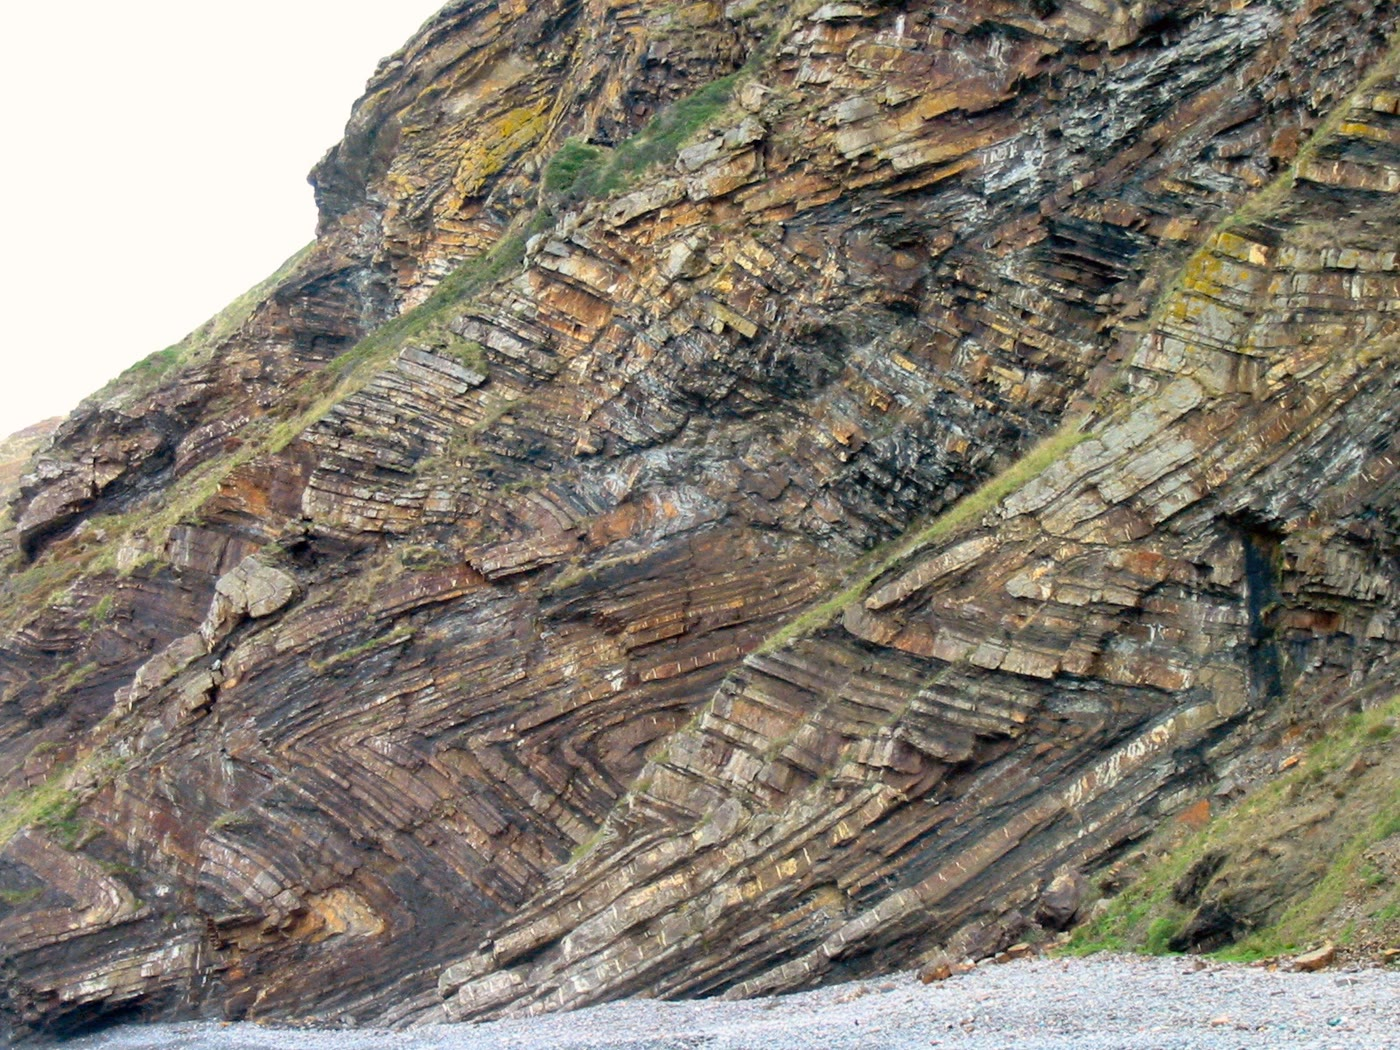
\includegraphics[width=0.78\linewidth]{images/book3/b1-chevron-folds-millook.jpg}
\par\smallskip{\small Lapisan batupasir dan batulanau yang terlipat di tebing-tebing Millook, North Cornwall: \omterm{def:b1:geological-maps:fold}{lipatan} zigzag dengan \omterm{def:b1:faults-folds-fabrics:fold-elements}{sayap} yang hampir lurus dan \omterm{def:b1:faults-folds-fabrics:fold-elements}{engsel} tajam, \omterm{def:b1:faults-folds-fabrics:fold-elements}{bidang aksialnya} hampir vertikal. Foto: Smalljim, CC~BY~3.0 (Wikimedia Commons).}
\label{fig:b1:faults-folds-fabrics:chevrons}
\end{omfigure}
% ledger: commons:millook

\section{Fabrik}\label{sec:b1:faults-folds-fabrics:fabrics}

Batuan yang terdeformasi sering kali terdeformasi di seluruh bagiannya, tidak hanya pada beberapa permukaan: butirannya diratakan, diputar atau tumbuh kembali ke dalam orientasi yang sama, yang memberinya fabrik. Fabrik planar membuat batuan terbelah, fabrik linear membuatnya pecah menjadi batang-batang.

\begin{definition}[Foliasi, skistositas, kleavage sabak, kleavage bidang-aksial]\label{def:b1:faults-folds-fabrics:foliation}
Sebuah \emph{foliasi}\index{foliasi} adalah fabrik planar yang meliputi batuan: sekumpulan permukaan sejajar yang berjarak rapat, dibuat oleh butiran pipih atau terratakan yang sejajar atau oleh lapisan-lapisan tipis, sepanjang mana batuan paling mudah terbelah. \emph{Skistositas}\index{skistositas} adalah foliasi batu sekis, dibuat oleh butiran sejajar yang lebih kasar daripada sekitar \qty{1}{mm}. \emph{Kleavage}\index{kleavage (batuan)} adalah foliasi batuan berbutir halus yang dibuat oleh deformasinya; \emph{kleavage sabak}\index{kleavage sabak} adalah kleavage batu sabak, dibuat oleh silikat berlapis yang terlalu kecil untuk dilihat dengan mata telanjang, dan terletak begitu rapat sehingga batuan dapat terbelah hampir di mana saja menjadi lembaran tipis. \emph{Kleavage bidang-aksial}\index{kleavage bidang-aksial} adalah kleavage yang sejajar, atau hampir sejajar, dengan \omterm{def:b1:faults-folds-fabrics:fold-elements}{bidang aksial} \omterm{def:b1:geological-maps:fold}{lipatan} dalam batuan yang sama.
\end{definition}
% ledger: ws:fabrics

\omterm{def:b1:faults-folds-fabrics:foliation}{Foliasi} terbentuk kira-kira tegak lurus terhadap arah pemendekan terbesar, oleh pemutaran butiran pipih, pertumbuhan \omterm{def:b1:rock-forming-minerals:groups}{mika} baru, dan pelarutan butiran pada muka-muka yang paling kuat ditekan. \omterm{def:b1:faults-folds-fabrics:foliation}{Kleavage sabak} karenanya tidak ada hubungannya dengan perlapisan lumpur: ia mencatat peremasan. Ketika \omterm{def:b1:geological-maps:fold}{lipatan} dan kleavage tumbuh dalam pemendekan yang sama, kleavage berada dekat dengan \omterm{def:b1:faults-folds-fabrics:fold-elements}{bidang aksial} \omterm{def:b1:geological-maps:fold}{lipatan}, dan ia sedikit mengipas melintasinya, berkumpul atau menyebar menurut kekuatan setiap lapisan, seperti yang ditunjukkan foto di bawah.
% ledger: ws:fabrics

\begin{omfigure}
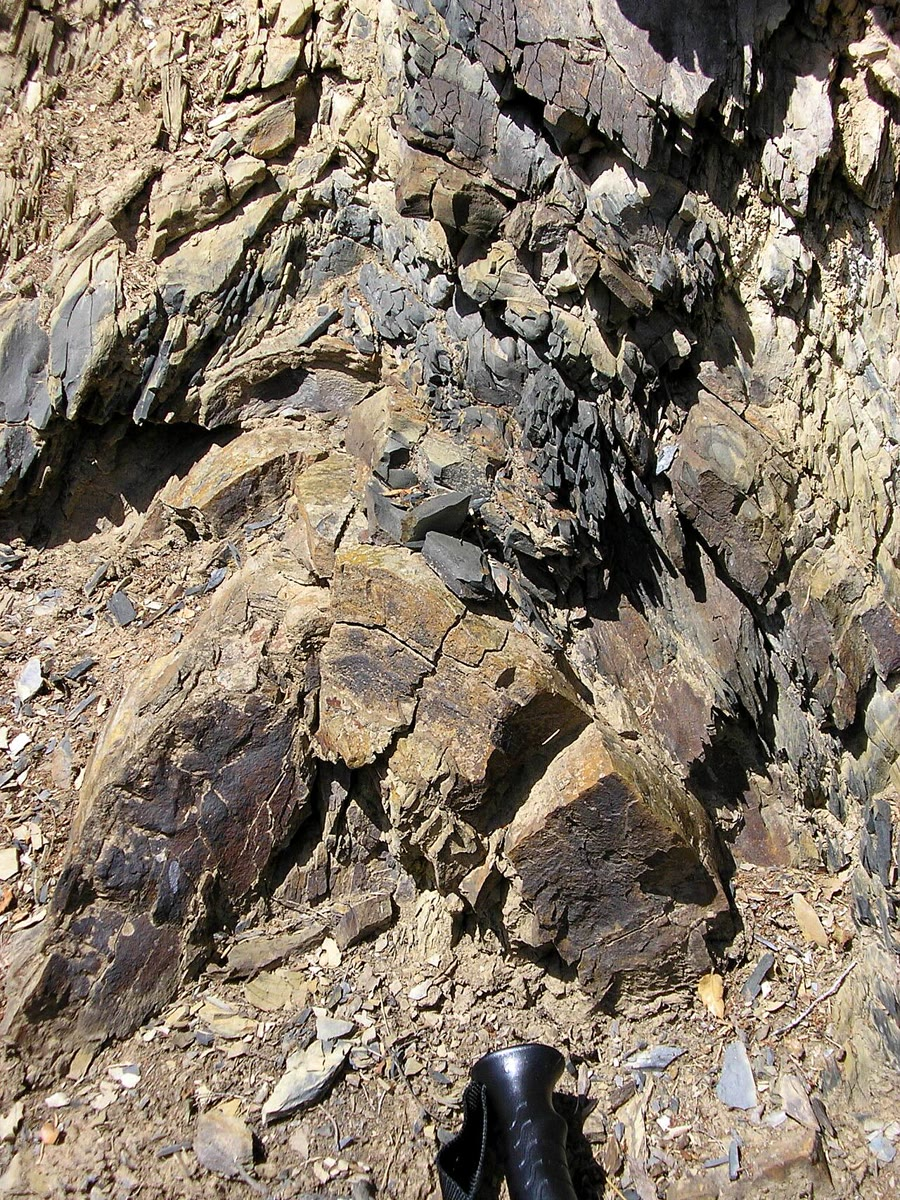
\includegraphics[height=8.2cm]{images/book3/b1-axial-planar-cleavage.jpg}
\par\smallskip{\small \omterm{def:b1:geological-maps:fold}{Antiklin} kecil dalam batupasir dan batulanau yang berselang-seling berumur Karbon, dekat Potes, Cantabria. Lapisan batupasir cokelat melengkung di atas \omterm{def:b1:faults-folds-fabrics:fold-elements}{engsel} di bagian tengah bawah gambar; dalam batulanau gelap di atasnya kleavage, sekumpulan rekahan curam dan berjarak rapat yang memotong lapisan, adalah bidang-aksial: hampir sejajar dengan \omterm{def:b1:faults-folds-fabrics:fold-elements}{bidang aksial} \omterm{def:b1:geological-maps:fold}{lipatan}, ia mengipas melintasinya, kipas itu berubah dari lapisan ke lapisan. Gagang tongkat jalan berdiameter sekitar \qty{4}{cm}. Foto: Mikenorton, CC~BY-SA~3.0 (Wikimedia Commons).}
\label{fig:b1:faults-folds-fabrics:cleavage}
\end{omfigure}
% ledger: commons:axial-cleavage

\begin{definition}[Lineasi, lineasi perpotongan, lineasi peregangan]\label{def:b1:faults-folds-fabrics:lineation}
Sebuah \emph{lineasi}\index{lineasi} adalah fabrik linear yang meliputi batuan, diukur dengan \omterm{def:b1:geological-maps:attitude}{jurus} dan \omterm{def:b1:field-lab-methods-1:trend-plunge}{penunjamannya}. \emph{Lineasi perpotongan}\index{lineasi perpotongan} adalah himpunan garis tempat dua fabrik planar saling memotong, seperti perlapisan dan kleavage; \emph{lineasi peregangan}\index{lineasi peregangan} terbuat dari butiran atau kerikil yang tertarik memanjang sepanjang arah peregangan terbesar.
\end{definition}
% ledger: ws:fabrics

\begin{proposition}[Lineasi perpotongan sebuah lipatan]\label{prop:b1:faults-folds-fabrics:intersection}
Dalam \omterm{def:b1:faults-folds-fabrics:fold-elements}{lipatan silindris} dengan \omterm{def:b1:faults-folds-fabrics:foliation}{kleavage bidang-aksial}, \omterm{def:b1:faults-folds-fabrics:lineation}{lineasi perpotongan} perlapisan dan kleavage sejajar dengan \omterm{def:b1:faults-folds-fabrics:fold-elements}{garis engsel}, di seluruh \omterm{def:b1:geological-maps:fold}{lipatan}.
\end{proposition}

\begin{proof}
Setiap permukaan perlapisan \omterm{def:b1:faults-folds-fabrics:fold-elements}{lipatan silindris} memuat arah sumbunya. \omterm{def:b1:faults-folds-fabrics:fold-elements}{Bidang aksial} memuat garis-garis \omterm{def:b1:faults-folds-fabrics:fold-elements}{engsel}, yang sejajar dengan sumbu, sehingga ia juga memuat arah itu, dan begitu pula setiap bidang kleavage yang sejajar dengannya. Dua bidang yang tidak sejajar dan keduanya memuat arah yang sama bertemu sepanjang garis dengan arah itu.
\end{proof}

Proposisi ini adalah jalan geolog lapangan menuju \omterm{def:b1:field-lab-methods-1:trend-plunge}{penunjaman} \omterm{def:b1:geological-maps:fold}{lipatan} yang terlalu besar untuk dilihat secara utuh: pada \omterm{def:b1:geological-maps:geological-map}{singkapan} mana pun dari salah satu \omterm{def:b1:faults-folds-fabrics:fold-elements}{sayapnya}, garis-garis tempat kleavage memotong perlapisan memberi \omterm{def:b1:faults-folds-fabrics:fold-elements}{garis engsel}. Perlapisan dan kleavage bersama-sama mengatakan lebih banyak: di mana \omterm{def:b1:geological-maps:fold}{lipatan} itu berada, dan lapisan menghadap ke arah mana.

\begin{definition}[Vergensi]\label{def:b1:faults-folds-fabrics:vergence}
\emph{Vergensi}\index{vergensi} sebuah \omterm{def:b1:geological-maps:fold}{lipatan} asimetris adalah arah horizontal ke arah mana bagian atasnya telah bergerak relatif terhadap bagian bawahnya: arah tempat ia terbalik atau, untuk \omterm{def:b1:faults-folds-fabrics:fold-classes}{lipatan miring}, ke arah mana ia condong.
\end{definition}
% ledger: ws:vergence

\begin{proposition}[Perlapisan dan kleavage pada sayap sebuah lipatan]\label{prop:b1:faults-folds-fabrics:cleavage-bedding}
Perhatikan sebuah \omterm{def:b1:geological-maps:fold}{lipatan} dengan \omterm{def:b1:faults-folds-fabrics:fold-elements}{sayap} lurus dan \omterm{def:b1:faults-folds-fabrics:foliation}{kleavage bidang-aksial}, dalam batuan yang tegak lurus dengan benar sebelum terlipat, dan di mana kedua \omterm{def:b1:faults-folds-fabrics:fold-elements}{sayap} turun dari setiap \omterm{def:b1:faults-folds-fabrics:fold-elements}{engsel} \omterm{def:b1:geological-maps:fold}{antiklin}. Dilihat dalam profil:
\begin{enumerate}[label=(\alph*)]
  \item pada \omterm{def:b1:faults-folds-fabrics:fold-elements}{sayap} tempat perlapisan dan kleavage miring ke arah yang sama, perlapisan itu lebih curam dari keduanya tepat ketika \omterm{def:b1:faults-folds-fabrics:fold-elements}{sayap} itu terbalik;
  \item rotasi lancip yang memutar kleavage ke perlapisan memiliki arah yang berlawanan pada kedua \omterm{def:b1:faults-folds-fabrics:fold-elements}{sayap} sebuah \omterm{def:b1:geological-maps:fold}{lipatan}; pada \omterm{def:b1:faults-folds-fabrics:fold-elements}{sayap} yang tidak terbalik, ia menggerakkan bagian atas kleavage secara horizontal ke arah \omterm{def:b1:faults-folds-fabrics:fold-elements}{engsel} \omterm{def:b1:geological-maps:fold}{antiklin} di bagian atas \omterm{def:b1:faults-folds-fabrics:fold-elements}{sayap} itu.
\end{enumerate}
\end{proposition}

\begin{proof}
Lihat sepanjang \omterm{def:b1:faults-folds-fabrics:fold-elements}{engsel} dengan \omterm{def:b1:faults-folds-fabrics:fold-elements}{bidang aksial} miring ke kiri pada sudut $\gamma$, $0 < \gamma \le \ang{90}$, dan hitung sudut berlawanan arah jarum jam dari horizontal yang menunjuk ke kanan. \omterm{def:b1:faults-folds-fabrics:foliation}{Kleavage}, sejajar dengan \omterm{def:b1:faults-folds-fabrics:fold-elements}{bidang aksial}, naik pada sudut $\gamma$. Pada \omterm{def:b1:faults-folds-fabrics:fold-elements}{engsel} \omterm{def:b1:geological-maps:fold}{antiklin} kedua \omterm{def:b1:faults-folds-fabrics:fold-elements}{sayap} turun dengan sudut $\ang{180} + \gamma - \iota/2$ (\omterm{def:b1:faults-folds-fabrics:fold-elements}{sayap}~1) dan $\ang{180} + \gamma + \iota/2$ (\omterm{def:b1:faults-folds-fabrics:fold-elements}{sayap}~2), di kedua sisi \omterm{def:b1:faults-folds-fabrics:fold-elements}{bidang aksial}, dengan $\iota/2 \le \gamma$ karena keduanya turun; setiap \omterm{def:b1:faults-folds-fabrics:fold-elements}{sayap} dari sebuah rangkaian \omterm{def:b1:geological-maps:fold}{lipatan} adalah salah satu dari dua ini untuk \omterm{def:b1:geological-maps:fold}{antiklin} di puncaknya. Batuan menjadi lebih muda ke luar, menjauhi inti \omterm{def:b1:geological-maps:fold}{antiklin}, sepanjang normal \omterm{def:b1:faults-folds-fabrics:fold-elements}{sayap} yang menunjuk menjauhi \omterm{def:b1:faults-folds-fabrics:fold-elements}{bidang aksial}.

\omterm{def:b1:faults-folds-fabrics:fold-elements}{Sayap}~1 turun ke kiri: ia miring ke kiri pada $\gamma - \iota/2$, kurang curam daripada kleavage. Normal keluarnya, pada $\ang{90} + \gamma -
\iota/2$, menunjuk ke atas: ia tegak dengan benar. Berjalan ke atas, ia membentuk sudut $\gamma - \iota/2$, sehingga rotasi lancip dari kleavage ke perlapisan searah jarum jam, sebesar $\iota/2$: bagian atas kleavage bergerak ke kanan, tempat \omterm{def:b1:faults-folds-fabrics:fold-elements}{engselnya} berada, karena \omterm{def:b1:faults-folds-fabrics:fold-elements}{sayap} itu meninggalkan \omterm{def:b1:faults-folds-fabrics:fold-elements}{engsel} ke kiri.

\omterm{def:b1:faults-folds-fabrics:fold-elements}{Sayap}~2 membentuk sudut $\gamma + \iota/2$ dengan horizontal, ke atas. Jika $\gamma + \iota/2 > \ang{90}$, ia turun ke kanan dan miring ke kanan, berlawanan dengan kleavage; normal keluarnya, pada $\ang{270} + \gamma +
\iota/2$, memiliki komponen ke atas $-\cos(\gamma + \iota/2) > 0$: ia tegak dengan benar. Jika $\gamma + \iota/2 < \ang{90}$, ia turun ke kiri, miring ke kiri pada $\gamma + \iota/2$, lebih curam daripada kleavage, dan komponen yang sama bernilai negatif: \omterm{def:b1:faults-folds-fabrics:fold-elements}{sayap} itu terbalik. Pada kedua kasus rotasi lancip dari kleavage ke perlapisan berlawanan arah jarum jam, sebesar $\iota/2$, dan menggerakkan bagian atas kleavage ke kiri; ketika \omterm{def:b1:faults-folds-fabrics:fold-elements}{sayap} itu tegak dengan benar ia meninggalkan \omterm{def:b1:faults-folds-fabrics:fold-elements}{engsel} ke kanan, sehingga \omterm{def:b1:faults-folds-fabrics:fold-elements}{engselnya} di kiri. \omterm{def:b1:faults-folds-fabrics:fold-elements}{Sayap} yang miring ke arah yang sama dengan kleavage dengan demikian adalah \omterm{def:b1:faults-folds-fabrics:fold-elements}{sayap}~1, yang lebih landai, dan \omterm{def:b1:faults-folds-fabrics:fold-elements}{sayap}~2 yang terbalik, yang lebih curam, yaitu (a); arah rotasinya searah jarum jam pada \omterm{def:b1:faults-folds-fabrics:fold-elements}{sayap}~1 dan berlawanan arah jarum jam pada \omterm{def:b1:faults-folds-fabrics:fold-elements}{sayap}~2, yaitu (b).
\end{proof}

Arah rotasi karenanya berubah di setiap \omterm{def:b1:faults-folds-fabrics:fold-elements}{engsel}, \omterm{def:b1:geological-maps:fold}{antiklin} maupun \omterm{def:b1:geological-maps:fold}{sinklin}. Seorang geolog yang mencatatnya di sepanjang lintasan menemukan \omterm{def:b1:faults-folds-fabrics:fold-elements}{engsel} \omterm{def:b1:geological-maps:fold}{lipatan} yang terlalu besar untuk dilihat dalam satu \omterm{def:b1:geological-maps:geological-map}{singkapan} di tempat arah berubah, dan \omterm{def:b1:faults-folds-fabrics:fold-elements}{sayap-sayap} terbalik di tempat perlapisan lebih curam daripada kleavage; kata \omterm{def:b1:faults-folds-fabrics:vergence}{vergensi} juga dipakai untuk arah rotasi ini, dan pembalikan \omterm{def:b1:faults-folds-fabrics:vergence}{vergensi} \omterm{def:b1:geological-maps:fold}{lipatan} kecil dipetakan dengan cara yang sama untuk menemukan \omterm{def:b1:faults-folds-fabrics:fold-elements}{engsel} \omterm{def:b1:geological-maps:fold}{lipatan} besar: \omterm{def:b1:geological-maps:fold}{lipatan-lipatan} kecil pada kedua \omterm{def:b1:faults-folds-fabrics:fold-elements}{sayap} sebuah \omterm{def:b1:geological-maps:fold}{lipatan} besar memiliki asimetri yang berlawanan, dan jejak aksialnya berjalan di antara keduanya.
% ledger: ws:vergence, ws:fold-elements

\begin{omfigure}
\begin{tikzpicture}[>={Stealth[length=5pt]}, font=\small]
% a train of chevron folds seen along the hinge (north into the page, east to the right):
% axial planes dipping 60 deg to the west, interlimb angle 40 deg; long limbs dip 40 deg W
% (the right way up), short limbs 80 deg W (overturned). Short limb: from an anticline hinge H_k,
% length s along 260 deg to the syncline hinge S_k; long limb back up along 40 deg to H_{k+1},
% so that all anticline hinges are level, a wavelength w apart.
% Five bedding surfaces, repeated along the axial direction (similar folds); cleavage parallel to it.
\def\s{2.6}
\pgfmathsetmacro{\sx}{\s*cos(260)}\pgfmathsetmacro{\sy}{\s*sin(260)}
\pgfmathsetmacro{\w}{\sx - \sy/tan(40)}
\pgfmathsetmacro{\hx}{0.62*cos(60)}\pgfmathsetmacro{\hy}{0.62*sin(60)}
\newcommand{\surface}[1]{%
  (-\w+#1*\hx, #1*\hy) \foreach \k in {-1,0,1,2,3} { -- ({\k*\w+\sx+#1*\hx}, {\sy+#1*\hy}) -- ({(\k+1)*\w+#1*\hx}, {#1*\hy}) }}
\begin{scope}
  \clip (0.35,-3.3) rectangle (10.0,2.95);
  \begin{scope}
    \clip \surface{0} -- (12,6) -- (-4,6) -- cycle;
    \clip \surface{4} -- (12,-6) -- (-4,-6) -- cycle;
    \fill[omLithSand!45] (-4,-6) rectangle (12,6);
    \fill[omLithShale!40] \surface{2} -- (12,6) -- (-4,6) -- cycle;
    \fill[omLithSand!45] \surface{3} -- (12,6) -- (-4,6) -- cycle;
    \foreach \c in {-8.0,-7.78,...,13.0} {
      \draw[omDef!85, line width=0.35pt] ({\c-6*cot(60)},-6) -- ({\c+6*cot(60)},6);
    }
  \end{scope}
  \foreach \j in {0,1,2,3,4} { \draw[line width=0.75pt, line join=round] \surface{\j}; }
\end{scope}
% axial traces through the anticline hinges, and labels
\foreach \k in {1,2,3} {
  \draw[omThm, dashed, line width=0.6pt] ({\k*\w-0.5*cos(60)},{-0.5*sin(60)}) -- ({\k*\w+3.6*cos(60)},{3.6*sin(60)});
  \node[omThm, font=\scriptsize, anchor=south] at ({\k*\w+3.6*cos(60)},{3.6*sin(60)}) {antiklin};
}
\foreach \k in {1,2,3} { \node[omThm, font=\scriptsize, anchor=north] at ({\k*\w+\sx},{\sy-0.15}) {sinklin}; }
\end{tikzpicture}
\par\smallskip{\small Satu rangkaian \omterm{def:b1:geological-maps:fold}{lipatan} zigzag yang terbalik ke kanan, dalam profil, dengan \omterm{def:b1:faults-folds-fabrics:foliation}{kleavage bidang-aksial} (garis biru tipis), digambar sesuai skala: \omterm{def:b1:faults-folds-fabrics:fold-elements}{bidang aksial} miring \ang{60} ke kiri, \omterm{def:b1:faults-folds-fabrics:fold-elements}{sudut antar-sayap} \ang{40}. \omterm{def:b1:faults-folds-fabrics:fold-elements}{Sayap-sayap} panjang miring \ang{40} ke kiri, kurang curam daripada kleavage, dan tegak dengan benar; \omterm{def:b1:faults-folds-fabrics:fold-elements}{sayap-sayap} pendek miring \ang{80} ke kiri, lebih curam daripada kleavage, dan terbalik. Memutar kleavage ke perlapisan melalui sudut lancip searah jarum jam pada setiap \omterm{def:b1:faults-folds-fabrics:fold-elements}{sayap} panjang dan berlawanan arah jarum jam pada setiap \omterm{def:b1:faults-folds-fabrics:fold-elements}{sayap} pendek. \omterm{def:b1:geological-maps:fold}{Lipatan-lipatan} itu bervergensi ke kanan.}
\label{fig:b1:faults-folds-fabrics:vergence}
\end{omfigure}

\section{Mikrostruktur}\label{sec:b1:faults-folds-fabrics:micro}

Di bawah mikroskop, deformasi batuan tampak pada butirannya. Sebutir kuarsa yang dilengkungkan oleh peluncuran lambat kisi kristalnya tidak lagi padam sekaligus di antara polarisator bersilang: ketika meja berputar, pita gelap menyapu melintasinya, karena bagian-bagiannya menunjuk ke arah yang sedikit berbeda. Pemadaman bergelombang ini (\cref{ch:b1:optical-mineralogy}) menguat ketika zona geser didekati, karena cacat menumpuk dalam kisi kristal. Di tempat air hadir, butiran melarut pada muka-muka tempat mereka ditekan paling keras, dan materi yang larut diendapkan di tempat tegangannya lebih rendah, atau dibawa pergi: pelarutan tekanan ini memendekkan batuan pada suhu rendah dan membangun banyak kleavage. Pada suhu yang lebih tinggi, butiran yang tertegang digantikan, sementara deformasi berlanjut, oleh butiran baru yang lebih kecil dan tidak tertegang, pertama-tama sepanjang batas butiran lama: rekristalisasi dinamis, yang mengecilkan ukuran butiran dan membuat \omterm{def:b1:faults-folds-fabrics:fault-rocks}{milonit}. Bentuk butiran yang terdeformasi dan \omterm{def:b1:rock-forming-minerals:mineral}{mineral} yang tumbuh dalam bayangan mereka juga menunjukkan ke arah mana zona geser bergerak; indikator arah geser ini, dan mekanismenya sendiri, termasuk dalam volume Tahun ke-3.
% ledger: ws:microstructures, ws:fabrics

\section{Latihan}

\begin{exercise}[$\star$]\label{exo:b1:faults-folds-fabrics:1}
Namai setiap sesar dari \omterm{def:b1:faults-folds-fabrics:fault-elements}{rake} \omterm{def:b1:faults-folds-fabrics:fault-elements}{vektor gesernya}, bidang yang miring \ang{60}: (a) $r = \ang{-90}$; (b) $r = \ang{85}$; (c) $r = 0$; (d) $r = \ang{180}$; (e) $r = \ang{-40}$. (f) Apa yang akan disebut (b) jika \omterm{def:b1:geological-maps:attitude}{kemiringannya} \ang{25}?
% ledger: ar:rake, usgs:fault-types
\end{exercise}

\begin{exercise}[$\star$]\label{exo:b1:faults-folds-fabrics:2}
Sebuah \omterm{def:b1:faults-folds-fabrics:fault-types}{sesar normal} miring \ang{55}; pergeserannya murni \omterm{def:b1:geological-maps:attitude}{pergeseran-kemiringan}, dengan \omterm{def:b1:faults-folds-fabrics:fault-elements}{pergeseran bersih} \qty{300}{m}. Hitung lemparan dan pergeseran horizontalnya.
\end{exercise}

\begin{exercise}[$\star$]\label{exo:b1:faults-folds-fabrics:3}
Berikan \omterm{def:b1:faults-folds-fabrics:fold-elements}{sudut antar-sayap} dan kelas setiap \omterm{def:b1:faults-folds-fabrics:fold-classes}{lipatan tegak}, yang \omterm{def:b1:faults-folds-fabrics:fold-elements}{sayap-sayapnya} miring ke arah berlawanan: (a) \omterm{def:b1:faults-folds-fabrics:fold-elements}{sayap-sayap} miring \ang{35} dan \ang{35}; (b) \ang{70} dan \ang{75}; (c) \ang{85} dan \ang{88}.
% ledger: ws:fold-classes
\end{exercise}

\begin{exercise}[$\star$]\label{exo:b1:faults-folds-fabrics:4}
Sebuah batupasir memiliki \omterm{def:b1:stress-strain-rheology:coulomb}{sudut gesekan internal} \ang{35}. Mengikuti teori Anderson, pada sudut berapa \omterm{def:b1:faults-folds-fabrics:fault-types}{sesar normal} dan \omterm{def:b1:faults-folds-fabrics:fault-types}{sesar dorongnya} miring? Sudut apa yang dibentuk dua \omterm{def:b1:faults-folds-fabrics:fault-types}{sesar geser-mendatar} konjugat satu sama lain?
\end{exercise}

\begin{exercise}[$\star\star$]\label{exo:b1:faults-folds-fabrics:5}
Sebuah sesar memiliki sikap $090/50$, dan \omterm{def:b1:faults-folds-fabrics:fault-rocks}{gores garis} dengan \omterm{def:b1:faults-folds-fabrics:fault-elements}{rake} \ang{-30} di atasnya; \omterm{def:b1:faults-folds-fabrics:fault-elements}{pergeseran bersihnya} \qty{400}{m}. (a) Hitung komponen geser-mendatar dan \omterm{def:b1:geological-maps:attitude}{pergeseran-kemiringan}, lemparan dan pergeseran horizontal. (b) Tuliskan \omterm{def:b1:faults-folds-fabrics:fault-elements}{vektor geser} dalam komponen timur, utara dan atas, dan berikan \omterm{def:b1:geological-maps:attitude}{jurus} dan \omterm{def:b1:field-lab-methods-1:trend-plunge}{penunjamannya}. (c) Namai sesarnya.
\end{exercise}

\begin{exercise}[$\star\star$]\label{exo:b1:faults-folds-fabrics:6}
Dua \omterm{def:b1:faults-folds-fabrics:fault-types}{sesar geser-mendatar} vertikal dengan umur sama berjurus $020$ dan $080$. (a) Mengikuti Anderson, berikan arah $\sigma_1$, $\sigma_2$ dan $\sigma_3$, dan \omterm{def:b1:stress-strain-rheology:coulomb}{sudut gesekan internal} batuan. (b) Sesar mana yang \omterm{def:b1:faults-folds-fabrics:fault-types}{dekstral} dan mana yang \omterm{def:b1:faults-folds-fabrics:fault-types}{sinistral}? Berargumentasilah dari pemendekan sepanjang $\sigma_1$.
\end{exercise}

\begin{exercise}[$\star\star$]\label{exo:b1:faults-folds-fabrics:7}
Kedua \omterm{def:b1:faults-folds-fabrics:fold-elements}{sayap} sebuah \omterm{def:b1:faults-folds-fabrics:fold-elements}{lipatan silindris} memiliki sikap $120/40$ dan $260/30$. Dengan \cref{prop:b1:faults-folds-fabrics:hinge}, cari \omterm{def:b1:geological-maps:attitude}{jurus} dan \omterm{def:b1:field-lab-methods-1:trend-plunge}{penunjaman} \omterm{def:b1:faults-folds-fabrics:fold-elements}{garis engselnya}, \omterm{def:b1:faults-folds-fabrics:fold-elements}{sudut antar-sayapnya} dan kelasnya.
\end{exercise}

\begin{exercise}[$\star\star$]\label{exo:b1:faults-folds-fabrics:8}
Pada sebuah \omterm{def:b1:geological-maps:geological-map}{singkapan}, perlapisan memiliki sikap $040/30$ dan \omterm{def:b1:faults-folds-fabrics:foliation}{kleavage bidang-aksial} sikap $160/80$. Cari \omterm{def:b1:geological-maps:attitude}{jurus} dan \omterm{def:b1:field-lab-methods-1:trend-plunge}{penunjaman} \omterm{def:b1:faults-folds-fabrics:lineation}{lineasi perpotongan}. Apa yang dikatakannya tentang \omterm{def:b1:geological-maps:fold}{lipatan} itu?
\end{exercise}

\begin{exercise}[$\star\star$]\label{exo:b1:faults-folds-fabrics:9}
Sebuah sesar vertikal berjurus timur--barat. Sebuah dike vertikal berjurus utara--selatan memotongnya; di utara sesar dike itu ditemukan \qty{350}{m} ke timur dari tempatnya di selatan sesar. (a) Apakah sesarnya \omterm{def:b1:faults-folds-fabrics:fault-types}{dekstral} atau \omterm{def:b1:faults-folds-fabrics:fault-types}{sinistral}? (b) Jika \omterm{def:b1:faults-folds-fabrics:fault-rocks}{gores garisnya} horizontal, berapa \omterm{def:b1:faults-folds-fabrics:fault-elements}{pergeseran bersihnya}? (c) Jika sebaliknya mereka menunjam \ang{20} ke timur, berapa \omterm{def:b1:faults-folds-fabrics:fault-elements}{pergeseran bersih} dan komponen vertikal pergeseran, dan blok mana yang turun?
\end{exercise}

\begin{exercise}[$\star\star\star$]\label{exo:b1:faults-folds-fabrics:10}
Sebuah sesar tanpa \omterm{def:b1:stress-strain-rheology:coulomb}{kohesi} dan koefisien gesekan $\mu$ membentuk sudut $\theta$ dengan $\sigma_1$. (a) Tunjukkan bahwa ia tergelincir ketika \omterm{def:b1:stress-strain-rheology:principal}{tegangan utama} efektif mencapai rasio
\[
  \frac{\sigma_1'}{\sigma_3'} = \frac{1 + \mu\cot\theta}{1 - \mu\tan\theta} .
\]
(b) Dengan $\mu = 0.6$ dan $\sigma_1$ vertikal, hitung rasio untuk \omterm{def:b1:faults-folds-fabrics:fault-types}{sesar normal} yang miring \ang{60}, \ang{45} dan \ang{35}. (c) Tunjukkan bahwa \omterm{def:b1:faults-folds-fabrics:fault-types}{sesar normal} yang miring kurang dari sudut tertentu tidak pernah dapat tergelincir, dan hitung sudut itu. (d) Untuk $\mu = 0.6$ dan $\mu = 0.85$, berikan \omterm{def:b1:geological-maps:attitude}{kemiringan} \omterm{def:b1:faults-folds-fabrics:fault-types}{sesar normal} dan \omterm{def:b1:faults-folds-fabrics:fault-types}{sesar dorong} yang paling baik orientasinya.
\end{exercise}

\begin{exercise}[$\star\star\star$]\label{exo:b1:faults-folds-fabrics:11}
Sepanjang lintasan timur--barat melintasi \omterm{def:b1:geological-maps:fold}{lipatan} zigzag yang \omterm{def:b1:faults-folds-fabrics:fold-elements}{engselnya} berjurus utara, sebuah \omterm{def:b1:faults-folds-fabrics:foliation}{kleavage bidang-aksial} miring \ang{60} ke barat di mana-mana. Perlapisan miring \ang{40} B di stasiun A, \ang{80} B di stasiun B dan \ang{40} B di stasiun C, dari barat ke timur, dalam batuan yang tegak dengan benar sebelum terlipat. (a) Stasiun mana yang berada di \omterm{def:b1:faults-folds-fabrics:fold-elements}{sayap} terbalik? (b) Ke arah mana kleavage memutar ke perlapisan di setiap stasiun, dilihat menghadap utara? (c) Di mana \omterm{def:b1:faults-folds-fabrics:fold-elements}{engselnya}, dan mana yang \omterm{def:b1:geological-maps:fold}{antiklin}? (d) Cari \omterm{def:b1:faults-folds-fabrics:fold-elements}{sudut antar-sayap} dan sikap \omterm{def:b1:faults-folds-fabrics:fold-elements}{bidang aksial}, dan katakan ke arah mana \omterm{def:b1:geological-maps:fold}{lipatan-lipatan} itu bervergensi.
\end{exercise}

\begin{exercise}[$\star\star\star$]\label{exo:b1:faults-folds-fabrics:12}
Sebuah lapisan sepanjang $L_0$ dilipat menjadi rangkaian \omterm{def:b1:geological-maps:fold}{lipatan} zigzag simetris dengan \omterm{def:b1:faults-folds-fabrics:fold-elements}{sudut antar-sayap} $\iota$, dengan panjangnya tidak berubah. (a) Tunjukkan bahwa panjangnya yang diukur melintasi \omterm{def:b1:geological-maps:fold}{lipatan} menjadi $L_0\sin(\iota/2)$. (b) Pemendekan apa yang diwakili \omterm{def:b1:geological-maps:fold}{lipatan} zigzag dengan \omterm{def:b1:faults-folds-fabrics:fold-elements}{sudut antar-sayap} \ang{60}? (c) \omterm{def:b1:faults-folds-fabrics:fold-elements}{Sudut antar-sayap} mana yang sesuai dengan pemendekan sebesar \qty{30}{\percent}? (d) Sebuah rangkaian \omterm{def:b1:faults-folds-fabrics:fold-classes}{lipatan tegak} dengan \omterm{def:b1:faults-folds-fabrics:fold-elements}{sayap} miring \ang{12}: berapa pemendekannya?
\end{exercise}

\section{Masalah: struktur Varden Hills, diukur}

\begin{problem}[{Soal akhir pekan --- antiklin dan sesar normal Varden Hills, dari sikap bidang-bidangnya ke pergeseran pada sesar}]
\label{pb:b1:faults-folds-fabrics:1}
% values: calc/ch17.py; region: figdata/shared/region.py (limbs, plunge, fault)
Varden Hills terlipat menjadi sebuah \omterm{def:b1:geological-maps:fold}{antiklin}, yang sumbunya berjalan utara--selatan pada $x = \qty{3.5}{km}$, dan sebuah \omterm{def:b1:geological-maps:fold}{sinklin} \qty{4}{km} di timur darinya; keduanya memiliki \omterm{def:b1:faults-folds-fabrics:fold-elements}{sayap} bidang. Survei lapangan mengukur perlapisan pada \omterm{def:b1:faults-folds-fabrics:fold-elements}{sayap} timur \omterm{def:b1:geological-maps:fold}{antiklin} sebagai $080.7/12.2$ dan pada \omterm{def:b1:faults-folds-fabrics:fold-elements}{sayap} baratnya sebagai $279.3/12.2$. Tutupannya dipotong oleh \omterm{def:b1:faults-folds-fabrics:fault-types}{sesar normal} dengan sikap $120/60$, yang \omterm{def:b1:faults-folds-fabrics:fault-elements}{dinding gantungnya} bergerak turun sepanjang \omterm{def:b1:geological-maps:attitude}{kemiringan}, dengan lemparan \qty{200}{m}. Berikan sudut hingga \ang{0.1} dan panjang hingga \qty{0.1}{m}.

\medskip
\noindent\textbf{Bagian I --- Sayap-sayap.}
\begin{enumerate}
  \item Tuliskan normal satuan ke atas $\mathbf n_1$ (\omterm{def:b1:faults-folds-fabrics:fold-elements}{sayap} timur) dan $\mathbf n_2$ (\omterm{def:b1:faults-folds-fabrics:fold-elements}{sayap} barat) dalam komponen timur, utara dan atas.
  \item Hitung $\mathbf n_1\cdot\mathbf n_2$ dan sudut antara normal-normalnya.
  \item Turunkan \omterm{def:b1:faults-folds-fabrics:fold-elements}{sudut antar-sayap} \omterm{def:b1:geological-maps:fold}{antiklin}.
  \item Klasifikasikan \omterm{def:b1:geological-maps:fold}{antiklin} menurut sudut itu.
  \item Kedua \omterm{def:b1:faults-folds-fabrics:fold-elements}{sayap} miring \ang{12.2}. Mengapa \omterm{def:b1:faults-folds-fabrics:fold-elements}{sudut antar-sayapnya} tidak tepat $\ang{180} - 2\times\ang{12.2}$? Hitung \omterm{def:b1:cross-sections:apparent-dip}{kemiringan semu} salah satu \omterm{def:b1:faults-folds-fabrics:fold-elements}{sayap} dalam penampang vertikal timur--barat.
  \item \omterm{def:b1:geological-maps:fold}{Sinklin} berbagi \omterm{def:b1:faults-folds-fabrics:fold-elements}{sayap} timur \omterm{def:b1:geological-maps:fold}{antiklin}, dan \omterm{def:b1:faults-folds-fabrics:fold-elements}{sayap} timurnya sendiri sejajar dengan \omterm{def:b1:faults-folds-fabrics:fold-elements}{sayap} barat \omterm{def:b1:geological-maps:fold}{antiklin}. Berapa \omterm{def:b1:faults-folds-fabrics:fold-elements}{sudut antar-sayapnya}?
\end{enumerate}

\medskip
\noindent\textbf{Bagian II --- Garis engsel dan bidang aksial.}
\begin{enumerate}[resume]
  \item Hitung $\mathbf n_1\times\mathbf n_2$, dan \omterm{def:b1:geological-maps:attitude}{jurus} dan \omterm{def:b1:field-lab-methods-1:trend-plunge}{penunjaman} \omterm{def:b1:faults-folds-fabrics:fold-elements}{garis engselnya}.
  \item Berikan sikap \omterm{def:b1:faults-folds-fabrics:fold-elements}{bidang aksial}. Apakah \omterm{def:b1:geological-maps:fold}{antiklin} itu tegak, miring atau rebah?
  \item Berikan deskripsi lengkap \omterm{def:b1:geological-maps:fold}{lipatan}: keketatan, sikap \omterm{def:b1:faults-folds-fabrics:fold-elements}{bidang aksial}, \omterm{def:b1:field-lab-methods-1:trend-plunge}{penunjaman}.
  \item Pada \omterm{def:b1:geological-maps:geological-map}{peta geologi} \cref{ch:b1:geological-maps}, ke arah mana \omterm{def:b1:geological-maps:geological-map}{singkapan} \omterm{def:b1:geological-maps:fold}{antiklin} menutup, dan apa yang tersingkap di intinya?
  \item Serpih tutupan membawa \omterm{def:b1:faults-folds-fabrics:foliation}{kleavage bidang-aksial}. Berikan sikapnya, dan \omterm{def:b1:geological-maps:attitude}{jurus} dan \omterm{def:b1:field-lab-methods-1:trend-plunge}{penunjaman} \omterm{def:b1:faults-folds-fabrics:lineation}{lineasi perpotongannya} pada \omterm{def:b1:faults-folds-fabrics:fold-elements}{sayap} timur.
  \item Pada \omterm{def:b1:faults-folds-fabrics:fold-elements}{sayap} timur, ke arah mana kleavage memutar ke perlapisan, dilihat menghadap utara, dan di sisi mana \omterm{def:b1:faults-folds-fabrics:fold-elements}{engsel} \omterm{def:b1:geological-maps:fold}{antiklin} berada?
\end{enumerate}

\medskip
\noindent\textbf{Bagian III --- Sesar dan tegangannya.}
\begin{enumerate}[resume]
  \item Berikan \omterm{def:b1:geological-maps:attitude}{jurus} sesar dengan kaidah tangan kanan, dan katakan di sisi mana dari jejaknya \omterm{def:b1:faults-folds-fabrics:fault-elements}{dinding gantung} berada.
  \item \omterm{def:b1:stress-strain-rheology:principal}{Tegangan utama} mana yang vertikal ketika sesar terbentuk, menurut Anderson?
  \item Berikan arah kedua \omterm{def:b1:stress-strain-rheology:principal}{tegangan utama} horizontal.
  \item \omterm{def:b1:stress-strain-rheology:coulomb}{Sudut gesekan internal} apa yang disiratkan oleh \omterm{def:b1:geological-maps:attitude}{kemiringan}? \omterm{def:b1:stress-strain-rheology:coulomb}{Koefisien gesekan internal} apa?
  \item Berikan sikap himpunan sesar konjugat yang dapat dibuat oleh tegangan yang sama, dan sudut antara kedua himpunan.
  \item Apakah sesar itu paling baik orientasinya untuk tergelincir lagi di bawah rezim yang sama, dengan gesekan Byerlee 0.85?
\end{enumerate}

\medskip
\noindent\textbf{Bagian IV --- Pergeseran.}
\begin{enumerate}[resume]
  \item Berikan \omterm{def:b1:faults-folds-fabrics:fault-elements}{rake} \omterm{def:b1:faults-folds-fabrics:fault-elements}{vektor geser}, dan \omterm{def:b1:geological-maps:attitude}{jurus} serta \omterm{def:b1:field-lab-methods-1:trend-plunge}{penunjamannya}.
  \item Tuliskan vektor satuan pergeseran dalam komponen timur, utara dan atas.
  \item Hitung pergeseran horizontal sesar.
  \item Hitung komponen timur dan utara dari pergeseran horizontal \omterm{def:b1:faults-folds-fabrics:fault-elements}{dinding gantung}.
  \item Periksa bahwa \omterm{def:b1:faults-folds-fabrics:fault-elements}{pergeseran bersih} $L$, lemparan $h$ dan pergeseran horizontal $e$ memenuhi $L^2 = h^2 + e^2$, dan jelaskan mengapa.
  \item Hingga meter terdekat, berapa \omterm{def:b1:faults-folds-fabrics:fault-elements}{pergeseran bersih} pada sesar Varden?
\end{enumerate}
\end{problem}
